\documentclass[]{article}
\usepackage{lmodern}
\usepackage{amssymb,amsmath}
\usepackage{ifxetex,ifluatex}
\usepackage{fixltx2e} % provides \textsubscript
\ifnum 0\ifxetex 1\fi\ifluatex 1\fi=0 % if pdftex
  \usepackage[T1]{fontenc}
  \usepackage[utf8]{inputenc}
\else % if luatex or xelatex
  \ifxetex
    \usepackage{mathspec}
  \else
    \usepackage{fontspec}
  \fi
  \defaultfontfeatures{Ligatures=TeX,Scale=MatchLowercase}
\fi
% use upquote if available, for straight quotes in verbatim environments
\IfFileExists{upquote.sty}{\usepackage{upquote}}{}
% use microtype if available
\IfFileExists{microtype.sty}{%
\usepackage{microtype}
\UseMicrotypeSet[protrusion]{basicmath} % disable protrusion for tt fonts
}{}
\usepackage[margin=1in]{geometry}
\usepackage{hyperref}
\hypersetup{unicode=true,
            pdftitle={The utility of spatial model-based estimators of unobserved bycatch: future or folly?},
            pdfauthor={Brian C. Stock1, Eric J. Ward2, James T. Thorson3, Jason E. Jannot3, Brice X. Semmens1},
            pdfborder={0 0 0},
            breaklinks=true}
\urlstyle{same}  % don't use monospace font for urls
\usepackage{graphicx,grffile}
\makeatletter
\def\maxwidth{\ifdim\Gin@nat@width>\linewidth\linewidth\else\Gin@nat@width\fi}
\def\maxheight{\ifdim\Gin@nat@height>\textheight\textheight\else\Gin@nat@height\fi}
\makeatother
% Scale images if necessary, so that they will not overflow the page
% margins by default, and it is still possible to overwrite the defaults
% using explicit options in \includegraphics[width, height, ...]{}
\setkeys{Gin}{width=\maxwidth,height=\maxheight,keepaspectratio}
\IfFileExists{parskip.sty}{%
\usepackage{parskip}
}{% else
\setlength{\parindent}{0pt}
\setlength{\parskip}{6pt plus 2pt minus 1pt}
}
\setlength{\emergencystretch}{3em}  % prevent overfull lines
\providecommand{\tightlist}{%
  \setlength{\itemsep}{0pt}\setlength{\parskip}{0pt}}
\setcounter{secnumdepth}{0}
% Redefines (sub)paragraphs to behave more like sections
\ifx\paragraph\undefined\else
\let\oldparagraph\paragraph
\renewcommand{\paragraph}[1]{\oldparagraph{#1}\mbox{}}
\fi
\ifx\subparagraph\undefined\else
\let\oldsubparagraph\subparagraph
\renewcommand{\subparagraph}[1]{\oldsubparagraph{#1}\mbox{}}
\fi

%%% Use protect on footnotes to avoid problems with footnotes in titles
\let\rmarkdownfootnote\footnote%
\def\footnote{\protect\rmarkdownfootnote}

%%% Change title format to be more compact
\usepackage{titling}

% Create subtitle command for use in maketitle
\newcommand{\subtitle}[1]{
  \posttitle{
    \begin{center}\large#1\end{center}
    }
}

\setlength{\droptitle}{-2em}
  \title{The utility of spatial model-based estimators of unobserved bycatch:
future or folly?}
  \pretitle{\vspace{\droptitle}\centering\huge}
  \posttitle{\par}
  \author{Brian C. Stock\textsuperscript{1}, Eric J. Ward\textsuperscript{2},
James T. Thorson\textsuperscript{3}, Jason E. Jannot\textsuperscript{3},
Brice X. Semmens\textsuperscript{1}}
  \preauthor{\centering\large\emph}
  \postauthor{\par}
  \date{}
  \predate{}\postdate{}

\usepackage{setspace}
%\singlespacing
%\onehalfspacing
\doublespacing
\usepackage{lineno}
\linenumbers
\usepackage{booktabs}
\usepackage{longtable}
\usepackage{array}
\usepackage{multirow}
\usepackage[table]{xcolor}
\usepackage{wrapfig}
\usepackage{float}
\usepackage{colortbl}
\usepackage{pdflscape}
\usepackage{tabu}
\usepackage{threeparttable}
\usepackage{threeparttablex}
\usepackage[normalem]{ulem}
\usepackage{makecell}

\begin{document}
\maketitle

\(^1\)+1 425 919 7879,
\href{mailto:b1stock@ucsd.edu}{\nolinkurl{b1stock@ucsd.edu}},
\href{mailto:semmens@ucsd.edu}{\nolinkurl{semmens@ucsd.edu}}, Scripps
Institution of Oceanography, University of California, San Diego, La
Jolla, California 92093 USA\\
\(^2\)\href{mailto:eric.ward@noaa.gov}{\nolinkurl{eric.ward@noaa.gov}},
Conservation Biology Division, Northwest Fisheries Science Center,
National Marine Fisheries Service, National Oceanic and Atmospheric
Administration, 2725 Montlake Blvd E, Seattle WA, 98112, USA\\
\(^3\)\href{mailto:james.thorson@noaa.gov}{\nolinkurl{james.thorson@noaa.gov}},
\href{mailto:jason.jannot@noaa.gov}{\nolinkurl{jason.jannot@noaa.gov}},
Fisheries Resource and Monitoring Division, Northwest Fisheries Science
Center, National Marine Fisheries Service, National Oceanic and
Atmospheric Administration, 2725 Montlake Blvd E, Seattle WA, 98112,
USA\\

\subsection{Abstract}\label{abstract}

Quantifying effects of fishing on non-targeted (bycatch) species is an
important management and conservation issue. Bycatch estimates are
typically calculated using data collected by on-board observers, but
observer programs are costly and therefore often only cover a small
percentage of the fishery. The challenge is then to estimate bycatch for
the unobserved fishing activity. The status quo for most fisheries is to
assume the ratio of bycatch-to-effort is constant and multiply this
ratio times the effort in the unobserved activity (ratio estimator). We
used a dataset with 100\% observer coverage, 35,440 hauls from the U.S.
West Coast groundfish trawl fishery, to evaluate the ratio estimator
against methods that utilize fine-scale spatial information: generalized
additive models (GAMs) and random forests. Applied to 15 species
representing a range of bycatch rates, including spatial locations
improved model predictive ability, whereas including effort-associated
covariates generally did not. Random forests performed best for all
species (lower root mean square error), but were slightly biased
(overpredicting total bycatch). Thus, the choice of bycatch estimation
method involves a tradeoff between bias and precision, and which method
is optimal may depend on the species bycatch rate and how the estimates
are to be used.

\subsection{Keywords}\label{keywords}

bycatch estimation, fishing effort, ratio estimator, spatial model, GAM
(generalized additive model), random forest, bias-variance tradeoff,
U.S. west coast groundfish fishery

\subsection{Introduction}\label{introduction}

The incidental bycatch of non-targeted species by fisheries in the US
and around the world has been highlighted as an issue of both
conservation concern and fisheries inefficiency (Harrington \emph{et
al.}, 2005), and reducing or eliminating bycatch and incidental
mortality is a goal of many fisheries around the world. There are
several reasons why a species might be considered bycatch or discarded:
the species may be of little or no commercial value, the species may be
protected (e.g.~marine mammals, turtles, birds), the species may be
permitted to be caught but in a different fishery, or the quota for the
targeted species in a given time period may be exceeded. In addition to
making fisheries more efficient, reducing bycatch can have positive
socioeconomic benefits to fishers. Two such examples include: fisheries
remaining open longer (before bycatch quotas are met), and valuable
stocks rebuilding more quickly due to reductions in take of overfished
bycatch species (NMFS, 2016).

Quantifying the amount of bycatch or discards for a given fishery can be
challenging. One of the most reliable sources of information is the use
of onboard scientific observers. Because observer programs are typically
expensive, few fisheries around the world are able to maintain 100\%
observer coverage. Instead, a subset of fishing activities is typically
monitored (trips, vessels). Assuming these observed units are
representative of unobserved fishing, ratio estimators can be used to
expand the observed bycatch ratio (i.e.~the ratio of bycatch-to-effort)
to the remainder of the fishery. In situations where bycatch rates are
assumed to vary by strata (e.g.~by season, depth, or latitude), the
ratio estimator can be applied separately to each stratum and then
summed to generate a total index of bycatch,
\(\sum_{ s=1 }^{ S }{ \frac { { d }_{ s } }{ { r }_{ s } } } { R }_{ s }\),
where \({ d }_{ s }\) is the observed bycatch or discards for stratum
\emph{s}, \({ r }_{ s }\) is the retained observed catch for stratum
\emph{s} and \({ R }_{ s }\) is the total landed catch in stratum
\emph{s} (Cochran, 1963). Importantly, ratio estimators do not
incorporate a formal underlying statistical model (i.e.~are free of any
assumptions regarding data structure), and are thus sample-based
estimators, rather than model-based estimators (McCracken, 2000). These
stratified ratio estimators have been widely used around the world and
applied to estimates of both discards (Anderson and Clark, 2003; Amandè
\emph{et al.}, 2010b) and protected species (Rogan and Mackey, 2007).

Despite their widespread use, there are a number of potential issues in
applying ratio estimators to enumerate fleetwide bycatch. First, using
observed catches of target species or any other measure of effort
implicitly makes an assumption about a linear relationship between
non-target and target catches (Fonteneau and Richard, 2003). This may be
unrealistic, particularly as the distribution of catches of non-target
species is often zero-inflated, or has a small number of observations
containing extremely high values (Ortiz and Arocha, 2004; Rochet and
Trenkel, 2005). Second, for species with low bycatch rates in fisheries
with low observer coverage (i.e.~rare-event bycatch), it is common for
zero bycatch events to be observed in a given year (ratio estimator =
0), and when bycatch events are observed, the ratio estimator often
delivers implausibly high estimates (McCracken, 2004; Martin \emph{et
al.}, 2015). Third, the boundaries of strata used in a ratio estimator
can be somewhat arbitrary whenever post-stratified boundaries are used
(as is common in multispecies sampling designs). A fourth and related
point is that within each stratum, bycatch rates are assumed to be
uniform, while in reality they may vary by season, depth, or other
factors.

One of the biggest questions related to bycatch estimation is whether
model-based estimators that incorporate explicit spatial information
(beyond any implicit spatial information incorporated by strata) offer
any advantage over the widely used stratified ratio estimator. Like
fishery independent catch per unit effort (CPUE) data, fishery dependent
bycatch patterns are spatially correlated (Lewison \emph{et al.}, 2009).
Accounting for spatial correlation in model-based estimators has been
extensively summarized in the geostatistical literature (Grondona and
Cressie, 1991; e.g. Brus and de Gruijter, 1997). Similar comparisons
have recently been applied to index standardization of fisheries survey
data (Maunder and Punt, 2004). In the majority of cases, spatially
explicit model-based estimators have increased precision relative to
simpler estimators that assign observations to strata (Thorson and Ward,
2013; Shelton \emph{et al.}, 2014; Thorson \emph{et al.}, 2015). There
are a number of additional advantages of spatial models, including the
ability to better quantify shifts in distribution (Thorson \emph{et
al.}, 2016), and improved ability to identify fine scale hotspots of
high bycatch (Cosandey-Godin \emph{et al.}, 2014; Ward \emph{et al.},
2015). While the majority of these recent analyses of fishery dependent
data have relied on parametric methods (delta-GLMM models; Thorson and
Ward, 2013), semi- or non-parametric models such as generalized additive
models (GAMs) or random forests (RFs) have also been used to include
spatial variation (Winker \emph{et al.}, 2013; Li \emph{et al.}, 2015;
Thorson \emph{et al.}, 2015).

While recent work has included fishing location information in spatial
model-based estimates of bycatch (Orphanides, 2009), there is little
guidance on how to model spatiotemporal variation, and how different
spatial modeling approaches compare in their bias or precision against
the traditional ratio estimator. To evaluate these different bycatch
estimators, we developed a simulation study from observer data collected
from the West Coast Groundfish Observer Program (WCGOP) at the Northwest
Fisheries Science Center. While observers have been monitoring a portion
of trips in the groundfish fishery since 2002, since 2011 regulations
require an observer on every groundfish trip (100\% coverage). Thus,
years with 100\% coverage can be subsampled to generate smaller datasets
that can be used to expand estimates to the fleet total, and the
relative performance of different methods can be compared because the
true bycatch is known. We begin by using the entirety of the dataset to
test the ratio estimator assumption of a linear relationship between
bycatch and available metrics of fishing effort. Next, we use randomly
generated subsamples of the observer data to evaluate (1) the relative
performance of spatial model-based bycatch estimates against the
conventional stratified ratio estimator, and (2) the sensitivity of
model performance to varying levels of observer coverage.

\subsection{Methods}\label{methods}

\subsubsection{Fisheries observer data}\label{fisheries-observer-data}

To evaluate the performance of ratio estimators versus spatial
model-based estimates of fleet-wide bycatch, we used a dataset from the
United States with 100\% observer coverage, the West Coast Groundfish
Observer Program (WCGOP) of the Northwest Fisheries Science Center
(NWFSC, Bellman \emph{et al.}, 2010). The WCGOP monitors commercial
bottom trawls on the west coast of the USA, which primarily target
groundfish such as Dover sole (\emph{Microstomus pacificus}),
thornyheads (\emph{Sebastolobus spp.}), sablefish (\emph{Anoplopoma
fimbria}), and rockfish (\emph{Sebastes spp.}). The fishery moved to an
individual fishing quota (IFQ) system with 100\% observer coverage in
2011, and we used the 35,440 post-IFQ hauls (4,007 trips) observed from
2011-2015 in the area north of Cape Falcon, Oregon (45.77° N, Fig.
\ref{fig:effort}). In 2015, a small portion of the fleet began
experimenting with the use of electronic monitoring equipment in lieu of
an observer. We excluded any such trips from our analysis. Observers
recorded haul duration, location, date, time, depth, gear type, and
at-sea catch including at-sea discarded bycatch (for details see NWFSC,
2016). Because fishermen are permitted to land a low quota of valuable
non-target species under IFQ management, we only considered 15 species
that are exclusively discarded and cover wide ranges of bycatch rates
and levels of management concern (Table \ref{tab:species-list}). Species
such as Dungeness crab or Pacific halibut are of high value, but as each
are permitted in other fisheries, they are considered bycatch in the
groundfish fishery.

\subsubsection{Relationship between bycatch and
effort}\label{relationship-between-bycatch-and-effort}

While the stratified ratio estimator typically involves multiplying the
bycatch-to-target catch ratio by the total target catch within strata,
it is certainly possible to replace target catch with other metrics of
effort, such as haul duration. This may be advantageous if a linear
relationship exists between bycatch and haul duration, but not between
bycatch and target catch. To investigate whether there was a linear
relationship between bycatch and available metrics of fishing effort,
retained catch of target species (kg) and haul duration (minutes), we
fit log-log linear models for each species:
\[ log(\text{Bycatch}) = \alpha + \beta \ log(\text{Effort}) + \epsilon\]
\[ \epsilon \sim \mathcal{N}(0,\,\sigma^{2})\] The slope term,
\(\beta\), of a log-log linear model is the exponent of an assumed power
law, i.e:
\[ \text{Bycatch} = e^\alpha \ \text{Effort}^{\beta} \ e^\epsilon\]
Thus, if a linear relationship between bycatch and fishing effort
exists, the power law exponent should equal one (\(\beta = 1\)).
Exponents greater than one (\(\beta > 1\)) imply positive concavity and
exponents less than one (\(\beta < 1\)) imply negative concavity, while
\(\beta = 0\) if no relationship exists.

\subsubsection{Simulation design}\label{simulation-design}

We compared the performance of the stratified ratio estimator with three
spatial modeling frameworks: GAM, VAST, and RF. All analyses were
conducted using R v3.4.4 (R Core Team, 2018). We designed our data
sub-sampling experiment to calculate predictive performance by
cross-validation. We generated 200 `training' datasets with reduced
observer coverage (e.g.~20\%, 40\%), by sampling trips (collections of
hauls) without replacement from the complete dataset. We used trip as
the cross-validation sample unit because this mirrors sampling schemes
in observer programs with less than 100\% coverage (i.e.~observers are
placed on vessels on a trip-by-trip basis, and then observe all hauls
within the trip). These training datasets were generated once for all
species, so that models were evaluated against the same simulated
datasets. Hauls from unobserved trips were then used as the `test'
dataset to evaluate predictions. This repeated training/test split
procedure is also known as ``leave-group-out cross-validation'' or
``Monte Carlo cross-validation,'' and a set of 200 train/test splits is
recommended as a good sample size (Kuhn and Johnson, 2013).

\paragraph{Status quo: ratio
estimator}\label{status-quo-ratio-estimator}

We implemented the stratified ratio estimator as described in the
Introduction and Bellman \emph{et al.} (2010), where observed estimates
of bycatch in each strata are expanded based on the ratio of observed to
total effort (total target catch or haul duration) and total estimates
are generated as sums over strata (Cochran, 1963). An important note
from a modeling perspective is that the ratio estimator is stratified by
year (5 levels: 2011, 2012, 2013, 2014, 2015), season (two levels:
summer, winter), depth (three levels: 0-125, 126-250, \textgreater{} 250
fathoms), and bimonthly period (six levels: Jan-Feb, Mar-Apr, \ldots{} ,
Nov-Dec). Any stratum with zero sampled bycatch is expanded to predict
zero total bycatch in that stratum.

\paragraph{Spatial framework \#1: generalized additive models
(GAMs)}\label{spatial-framework-1-generalized-additive-models-gams}

We fit GAMs using two alternative methods of accounting for zeros. Our
first approach, the ``GAM-Delta'' model, partitioned the data into
separate presence/absence (`binomial') and `positive' components (a
delta, or hurdle, model as in Pennington, 1983; Maunder and Punt, 2004).
The GAM-Delta model estimates of total density were then calculated by
multiplying the binomial and positive components (as in Lo \emph{et
al.}, 1992). The second approach, the ``GAM-Tweedie'' model, treats zero
inflated catch data as arising from a Tweedie distribution with power
parameter \(1 < p < 2\), which is a compound Poisson process where catch
is modeled as the sum of \(N\) independent gamma random variables, with
\(N\) following a Poisson distribution (Tweedie, 1984). Assuming a
Tweedie distribution is reasonable, as the haul catch (weight) can be
thought of as a sum of the weight of \(N\) fish, where the weight of
each fish is gamma-distributed (Candy, 2004). Importantly, this allows
for hauls with zero catch, since \(N\) can be zero. We estimated the
Tweedie power parameter, \(p\), for each species outside the model using
maximum likelihood, and then fit GAMs using these fixed,
species-specific \(p\) values.

We fit both the GAM-Delta and GAM-Tweedie models using the `mgcv'
library (v1.8-17, Wood, 2006) and the same covariates as the ratio
estimator, adding a 2D thin plate regression spline on location:

\[ \text{bycatch} \sim \text{year} + \text{season} + \text{bimonth} + \text{bimonth}^2 + \text{depth interval} + \text{s}(\text{lat}, \text{long}, k=50) \]

Tensor product splines were also considered for the 2D spline, since
they are designed for cases where the scale differs in the two
dimensions (as in our case, along- vs.~cross-shore distance). We used
thin plate regression splines instead, however, because they had better
predictive performance in preliminary testing. We used the same factor
covariates as the ratio estimator (fixed effects of year, season,
bimonthly period, and depth interval) for two reasons. First, this
offered a more direct comparison between the ratio estimator and GAMs.
Second, this analysis aims to inform the process of producing yearly
bycatch estimates for dozens of species in a highly multispecies trawl
fishery, where lengthy model selection is impractical given current
logistical constraints (Bellman \emph{et al.}, 2010).

We fit four variations of each GAM model to determine the effect of
including location and effort on predictive performance: no effort or
location, location only, effort only, and both location and effort.

\paragraph{Spatial framework \#2: random forests
(RFs)}\label{spatial-framework-2-random-forests-rfs}

Similar to the GAMs, we fit two random forest models. ``RF-Delta''
considered the binomial and positive data independently and multiplied
them together to calculate total bycatch density. ``RF-Total'' treated
the binomial and positive data as occurring from the same process in a
single model.

We used `randomForest' (v4.6-12, Liaw and Wiener, 2002) to fit the RFs,
and we used the same covariates as the ratio estimator and GAMs, plus
linear and quadratic terms for location:

\[ \text{bycatch} \sim \text{year} + \text{season} + \text{bimonth} + \text{bimonth}^2 + \text{depth interval} + \text{lat} + \text{lat}^2 + \text{lon} + \text{lon}^2\]

Since RFs are claimed to not overfit data (Breiman, 2001) and suffer
less from incorporating numerous, possibly correlated and uninformative
covariates (Biau and Scornet, 2016), we fit a third RF model using all
available covariates without stratification. We expected this ``RF-All''
model to outperform the RF-Delta and RF-Total models because,
presumably, information is lost by not including covariates (haul number
in trip, gear, time of day) and stratifying depth (to depth interval),
date (to season and bimonthly period), and location (areas by latitude).
We included day-of-year and hour-of-day as periodic functions (i.e.
\(\text{sinhour} = sin \left[ \frac{2 \pi \text{hour}}{24} \right]\)):

\[ \text{bycatch} \sim \text{year} + \text{depth} + \text{haul number} + \text{gear} + \text{cosday} + \text{sinday} + \text{coshour} + \text{sinhour} + \text{lat} + \text{lat}^2 + \text{lon} + \text{lon}^2\]

\subsubsection{Model evaluation}\label{model-evaluation}

For each simulated dataset, we calculated model performance as root mean
square error (RMSE) using the predicted and observed bycatch. RMSE was
calculated by year, and also averaged across years. As RMSE can be
expressed as the sum of variance and squared bias, we also generated
estimates of the bias from each prediction, in order to better
understand the relative contributions to total RMSE (in other words, why
some models do better than others).

\subsection{Results}\label{results}

\subsubsection{Weak relationship between effort and
bycatch}\label{weak-relationship-between-effort-and-bycatch}

For nearly all of the 15 species included in our analysis, we found that
relationships between bycatch and effort (both target catch and haul
duration) were either weak or nonlinear, as most power law exponents
from the log-log regression were much less than 1 (25/30 \textless{}
0.5, Figs. \ref{fig:effort-bycatch-slopes}, \ref{fig:effort-bycatch},
and \ref{fig:effort-bycatch-2}). In only a few cases were the estimated
coefficients close to 1.0 (the relationship assumed when effort is
included as an offset).

\subsubsection{Model comparison: RF had lower error but slight
bias}\label{model-comparison-rf-had-lower-error-but-slight-bias}

Compared to the ratio estimator, we found that the RF-Total model (not
applying a hurdle or delta model) produced estimates of total bycatch
that had lower RMSE (26\% lower averaged across species, Fig.
\ref{fig:model-comparison}). For most species and years, median bycatch
estimates from the ratio estimator and RF-Total were close to each other
and the true, observed bycatch, but the RF-Total model was more precise
(Fig. \ref{fig:model-comparison-byyear-catch}). However, RF-Total had
higher bias compared to the ratio method (median percent error across
all species and years: RF = 0.068, Ratio = -0.011, Fig.
\ref{fig:model-comparison-byyear}). The GAM-Tweedie model appeared to
have convergence issues for some simulations in one-fifth of the species
(Black skate, California slickhead, and Grenadier), but for the
simulations that did converge, it performed similarly to the ratio
estimator (Fig. \ref{fig:model-comparison}).

Though delta models have been widely used in the index standardization
of fisheries data (Maunder and Punt, 2004), both GAM and RF models with
an aggregated response consistently outperformed delta models (Fig.
\ref{fig:model-comparison-delta}).

\subsubsection{Effect of including fishing effort and spatial
locations}\label{effect-of-including-fishing-effort-and-spatial-locations}

We found minimal gain in predictive performance when fishing effort was
included as a covariate. In all models compared, any effect of effort
was smaller than the effect of including spatial locations (Fig.
\ref{fig:covariate-effects}). An important difference between the GAM
and RF models was that for many species, adding spatial locations to
GAMs led to worse predictions, while adding location information to the
RF models either improved predictions (especially for RF-Delta) or had
no effect.

\subsubsection{Influence of data richness on model
performance}\label{influence-of-data-richness-on-model-performance}

As expected, model performance improved for higher observer coverage
(20\% vs.~40\%, Fig. \ref{fig:coverage-effects}). Averaged across
species, RF had markedly lower median RMSE than the ratio estimator. In
fact, the RF models based on 20\% observer coverage (0.155 median RMSE)
outperformed the ratio estimator based on 40\% observer coverage (0.180
median RMSE). Similarly, the performance advantage (indicated by lower
RMSE) of RF over the ratio estimator was most pronounced for species
with low bycatch rates, and decreased for species with higher bycatch
rates (Fig. \ref{fig:bycatch-rate-rmse}).

\subsection{Discussion}\label{discussion}

In terms of the relative performance across models, our results are
consistent with previous studies showing that non-parametric methods
such as random forests offer improved predictive capabilities over GAMs
and delta-GLMM models (Marmion \emph{et al.}, 2009; Knudby \emph{et
al.}, 2010; Rooper \emph{et al.}, 2017). Including the spatial location
of fishing offered a considerable improvement in RMSE for many species,
particularly in the RF-Delta modeling framework (Fig.
\ref{fig:covariate-effects}). However, once spatial information was
included, the addition of effort had a minimal effect in reducing RMSE.
This result is not surprising, given the weak relationships between
bycatch and effort revealed by our log-log analyses (Figs.
\ref{fig:effort-bycatch-slopes}, \ref{fig:effort-bycatch}, and
\ref{fig:effort-bycatch-2}). We found decreases in RMSE for all species
and models as observer coverage increased from 20\% to 40\% (Fig.
\ref{fig:coverage-effects}). The improvement in predictive capabilities
with increasing observer coverage is consistent with previous simulation
experiments using different fisheries (Babcock \emph{et al.}, 2003;
Amandè \emph{et al.}, 2010a).

For an observer program tasked with producing yearly bycatch estimates
for many species, the ideal bycatch estimation model is simple,
converges rapidly, performs well on average, and never performs much
worse than a default option like a ratio estimator. Therefore, the fact
that RF had equal or lower prediction error than the ratio estimator for
all species and scenarios is an important finding. The desire for one
simple model also informed our selection of candidate models; we did not
test an exhaustive list of modeling options for spatiotemporal bycatch
data, but a subset of models that analysts are familiar with and can
apply quickly. We assumed that each species in our simulations were
affected by the same set of covariates; ideally, a single best model
could be developed for each species in a given fishery, with unique
covariates. We also restricted covariates in our analysis to the same
information that is typically used in the ratio estimator, even though
some covariates (e.g.~depth, date of year) could be treated as
continuous rather than discrete factor variables. However, including all
available covariates without stratification in a RF model, RF-All,
actually performed worse than the model with fewer, stratified
covariates, RF-Total (Fig. \ref{fig:model-comparison-delta}). While RF
are touted as robust to overfitting and the inclusion of noninformative
covariates (Breiman, 2001; Biau and Scornet, 2016), one possible
explanation for this result is that RF-All did overfit the data.

The second important finding from our simulations with practical
implications for management is that the choice of one estimator over
another is accompanied by an implicit tradeoff between bias and
variance. While RF had equal or lower prediction error than the ratio
estimator for all species, RF was slightly biased high (overestimating
true bycatch, Fig. \ref{fig:model-comparison-byyear}). On the other
hand, RF estimates were much less variable than the ratio estimator.
This bias-variance tradeoff was apparent for all species in our
simulations (Fig. \ref{fig:variance-bias}), but depended on the species'
bycatch rate (Fig. \ref{fig:bycatch-rate-rmse}). For commonly-caught
species like Sandpaper skate or Brown cat shark, where RF and the ratio
estimator had similar RMSE, RF offered slight reductions in uncertainty
but had large increases in bias. For rarely-caught species, like
California slickhead or Dungeness crab, RF exchanged large reductions in
uncertainty for modest increases in bias. The recommendation of one
methodology over another largely depends on what the bycatch estimates
will be used for. Stock assessment scientists, for example, may be
largely interested in unbiased but imprecise estimates, such as the
ratio estimator, which can then be fitted and smoothed statistically
during model fitting. On the other hand, scientists or policy makers who
are more concerned about relative changes in bycatch over time may
prefer more precise estimators (such as RF) that are more robust to
noise arising from sampling less than 100\% of the fishery. We recommend
further research regarding circumstances when it is important to
minimize bias versus imprecision when processing data for inclusion in a
second-stage model (Szpiro and Paciorek, 2013).

The bias of a RF model is roughly equal to the bias of the individual
regression trees it comprises, so it should not be expected to produce
unbiased estimates (Breiman, 1999; Kuhn and Johnson, 2013; Xu, 2013). RF
bias depends on the response variable distribution--RF will be unbiased
for a uniform response, and we can expect positive bias for typical
fisheries catch distributions (positive, right-skewed). Why? Consider
how each individual tree in a RF generates predictions for the tails of
a distribution. Terminal nodes for extreme values use the mean of the
training data in those nodes, so trees tend to overpredict in the lower
tail and underpredict in the upper tail. Because bycatch is
right-skewed, there are more observations in the lower tail, and
therefore more overprediction than underprediction. Several bias
correction methods have been proposed, and we tested two: 1) Cubist,
which fits a linear model in terminal nodes instead of using the data
mean (Quinlan, 1992, 1993), and 2) Xu (2013), which fits a second RF
model to the residuals of the original RF. Unfortunately, Cubist reduced
but did not eliminate bias, and Xu (2013) performed poorly (e.g.~for
Dungeness crab, Cubist reduced median percent error from 0.055 to 0.043,
Fig. \ref{fig:rf-cubist}).

Based on the results from our simulation study, there are several
potential avenues of future research that will help to advance the
inclusion of spatial information into bycatch estimation. First,
additional work could be done to improve variance estimation for
non-parametric methods such as RF. Resampling or bootstrapped estimates
could be generated for fisheries with less than 100\% observer coverage,
and variance estimates could be compared to analytic estimates via the
ratio estimator (Cochran, 1963). Second, it may be useful to perform a
more detailed comparison between the models used here, and the
spatiotemporal delta-GLMM models that have been widely used for
fisheries survey data (Thorson \emph{et al.}, 2015). Similarly,
multispecies spatiotemporal models may improve predictions of local
density by sharing information about underlying spatial patterns
(Latimer \emph{et al.}, 2009; Warton \emph{et al.}, 2015; Ovaskainen
\emph{et al.}, 2016; Thorson and Barnett, 2017; Thorson \emph{et al.},
2017). Additionally, advice on the number and distribution of knots or
random effects in spatiotemporal models would be useful for analysts
interested in applying these models.

\subsection{Supplementary material}\label{supplementary-material}

The following supplementary material is available online:

Table S1 - Figure S1 - Figure S2 - Figure S3 - Figure S4 - Figure S5 -

\subsection{Acknowledgements}\label{acknowledgements}

BCS received support from the National Science Foundation Graduate
Research Fellowship under Grant No. DGE-1144086, as well as a Graduate
Research Internship Program allowance. The authors thank the WCGOP staff
at the NWFSC, and the dedicated observers who made this work possible.

\subsection{References}\label{references}

\hypertarget{refs}{}
\hypertarget{ref-amande2010b}{}
Amandè, M., Lennert-Cody, C., Bez, N., Hall, M., and Chassot, E. 2010a.
How much sampling coverage affects bycatch estimates in purse seine
fisheries. IOTC-2010-WPEB-20. Working Party on Ecosystem; Bycatch.

\hypertarget{ref-amande2010a}{}
Amandè, M. J., Ariz, J., Chassot, E., de Molina, A. D., Gaertner, D.,
Murua, H., and Pianet, R. \emph{et al.} 2010b. Bycatch of the European
purse seine tuna fishery in the Atlantic Ocean for the 2003--2007
period. Aquatic Living Resources, 23: 353--362.

\hypertarget{ref-anderson2003}{}
Anderson, O. F., and Clark, M. R. 2003. Analysis of bycatch in the
fishery for orange roughy, \emph{Hoplostethus atlanticus}, on the South
Tasman Rise. Marine and Freshwater Research, 54: 643--652.

\hypertarget{ref-babcock2003}{}
Babcock, E., Pikitch, E., and Hudson, C. 2003. How much observer
coverage is enough to adequately estimate bycatch? Oceana, 2501 M
Street, NW, Suite 300 Washington, DC 20037.

\hypertarget{ref-bellman2010}{}
Bellman, M. A., Heery, E., and Majewski, J. 2010. Observed and estimated
total bycatch of green sturgeon in the 2002-2008 U.S. West Coast
groundfish fisheries. West Coast Groundfish Observer Program, NWFSC,
2725 Montlake Blvd E., Seattle, WA.

\hypertarget{ref-biau2016}{}
Biau, G., and Scornet, E. 2016. A random forest guided tour. TEST, 25:
197--227.

\hypertarget{ref-breiman1999}{}
Breiman, L. 1999. Using adaptive bagging to debias regressions.
Technical Report 547. Statistics Dept. UCB.

\hypertarget{ref-breiman2001}{}
Breiman, L. 2001. Random forests. Machine Learning, 45: 5--32.

\hypertarget{ref-brus1997}{}
Brus, D. J., and de Gruijter, J. J. 1997. Random sampling or
geostatistical modelling? Choosing between design-based and model-based
sampling strategies for soil (with discussion). Geoderma, 80: 1--44.

\hypertarget{ref-candy2004}{}
Candy, S. G. 2004. Modelling catch and effort data using generalised
linear models, the Tweedie distribution, random vessel effects and
random stratum-by-year effects. CCAMLR Science, 11: 59--80.

\hypertarget{ref-cochran1963}{}
Cochran, W. 1963. Sampling techniques. J Wiley and Sons, New York, NY.

\hypertarget{ref-cosandey-godin2014}{}
Cosandey-Godin, A., Krainski, E. T., Worm, B., and Flemming, J. M. 2014.
Applying Bayesian spatiotemporal models to fisheries bycatch in the
Canadian Arctic. Canadian Journal of Fisheries and Aquatic Sciences, 72:
186--197.

\hypertarget{ref-fonteneau2003}{}
Fonteneau, A., and Richard, N. 2003. Relationship between catch, effort,
CPUE and local abundance for non-target species, such as billfishes,
caught by Indian Ocean longline fisheries. Marine and Freshwater
Research, 54: 383--392.

\hypertarget{ref-grondona1991}{}
Grondona, M. O., and Cressie, N. 1991. Using spatial considerations in
the analysis of experiments. Technometrics, 33: 381--392.

\hypertarget{ref-harrington2005}{}
Harrington, J. M., Myers, R. A., and Rosenberg, A. A. 2005. Wasted
fishery resources: Discarded by-catch in the USA. Fish and Fisheries, 6:
350--361.

\hypertarget{ref-knudby2010}{}
Knudby, A., Brenning, A., and LeDrew, E. 2010. New approaches to
modelling fish--habitat relationships. Ecological Modelling, 221:
503--511.

\hypertarget{ref-kuhn2013}{}
Kuhn, M., and Johnson, K. 2013. Applied predictive modeling. Springer
Science \& Business Media, New York, NY.

\hypertarget{ref-latimer2009}{}
Latimer, A. M., Banerjee, S., Sang Jr, H., Mosher, E. S., and Silander
Jr, J. A. 2009. Hierarchical models facilitate spatial analysis of large
data sets: A case study on invasive plant species in the northeastern
United States. Ecology Letters, 12: 144--154.

\hypertarget{ref-lewison2009}{}
Lewison, R. L., Soykan, C. U., and Franklin, J. 2009. Mapping the
bycatch seascape: Multispecies and multi-scale spatial patterns of
fisheries bycatch. Ecological Applications, 19: 920--930.

\hypertarget{ref-li2015}{}
Li, Z., Ye, Z., Wan, R., and Zhang, C. 2015. Model selection between
traditional and popular methods for standardizing catch rates of target
species: A case study of Japanese Spanish mackerel in the gillnet
fishery. Fisheries Research, 161: 312--319.

\hypertarget{ref-liaw2002}{}
Liaw, A., and Wiener, M. 2002. Classification and regression by
randomForest. R News, 2: 18--22. \url{http://arxiv.org/abs/1609-3631}.

\hypertarget{ref-lo1992}{}
Lo, N. C. H., Jacobson, L. D., and Squire, J. L. 1992. Indices of
relative abundance from fish spotter data based on delta-lognormal
models. Canadian Journal of Fisheries and Aquatic Science, 49:
2515--2526.

\hypertarget{ref-marmion2009}{}
Marmion, M., Parviainen, M., Luoto, M., Heikkinen, R. K., and Thuiller,
W. 2009. Evaluation of consensus methods in predictive species
distribution modelling. Diversity and Distributions, 15: 59--69.

\hypertarget{ref-martin2015}{}
Martin, S. L., Stohs, S. M., and Moore, J. E. 2015. Bayesian inference
and assessment for rare-event bycatch in marine fisheries: a drift
gillnet fishery case study. Ecological Applications, 25: 416--429.

\hypertarget{ref-maunder2004}{}
Maunder, M. N., and Punt, A. E. 2004. Standardizing catch and effort
data: A review of recent approaches. Fisheries Research, 70: 141--159.

\hypertarget{ref-mccracken2000}{}
McCracken, M. L. 2000. Estimation of sea turtle take and mortality in
the Hawaiian longline fisheries. Honolulu Laboratory, Southwest
Fisheries Science Center, National Marine Fisheries Service, NOAA, 2570
Dole Street, Honolulu, Hawaii 96822-2396.

\hypertarget{ref-mccracken2004}{}
McCracken, M. L. 2004. Modeling a very rare event to estimate sea turtle
bycatch: lessons learned. U.S. Dep. Commer., NOAA Tech Memo.,
NMFS-TM-PIFSC-3.

\hypertarget{ref-nmfs2016bycatch}{}
NMFS. 2016. National bycatch reduction strategy. U.S. Dep. Commer.,
NOAA, Natl. Mar. Fish. Serv., Silver Spring, MD.

\hypertarget{ref-nwfsc2016}{}
(NWFSC) Northwest Fisheries Science Center. 2016. West Coast Groundfish
Observer Program 2016 catch shares training manual. West Coast
Groundfish Observer Program, NWFSC, 2725 Montlake Blvd E., Seattle, WA,
98112.

\hypertarget{ref-orphanides2009}{}
Orphanides, C. 2009. Protected species bycatch estimating approaches:
Estimating harbor porpoise bycatch in U. S. Northwestern Atlantic
gillnet fisheries. J. Northw. Atl. Fish. Sci., 42: 55--76.

\hypertarget{ref-ortiz2004}{}
Ortiz, M., and Arocha, F. 2004. Alternative error distribution models
for standardization of catch rates of non-target species from a pelagic
longline fishery: Billfish species in the Venezuelan tuna longline
fishery. Fisheries Research, 70: 275--297.

\hypertarget{ref-ovaskainen2016}{}
Ovaskainen, O., Roy, D. B., Fox, R., and Anderson, B. J. 2016.
Uncovering hidden spatial structure in species communities with
spatially explicit joint species distribution models. Methods in Ecology
and Evolution, 7: 428--436.

\hypertarget{ref-pennington1983}{}
Pennington, M. 1983. Efficient estimators of abundance, for fish and
plankton surveys. Biometrics, 39: 281--286.

\hypertarget{ref-quinlan1992}{}
Quinlan, J. R. 1992. Learning with continuous classes. \emph{In} 5th
australian joint conference on artificial intelligence, pp. 343--348.

\hypertarget{ref-quinlan1993}{}
Quinlan, J. R. 1993. Combining instance-based and model-based learning.
\emph{In} Proceedings of the tenth international conference on machine
learning, pp. 236--243.

\hypertarget{ref-rcoreteam2018}{}
R Core Team. 2018. R: A language and environment for statistical
computing. R Foundation for Statistical Computing, Vienna, Austria.
\url{https://www.R-project.org/}.

\hypertarget{ref-rochet2005}{}
Rochet, M. J., and Trenkel, V. M. 2005. Factors for the variability of
discards: Assumptions and field evidence. Canadian Journal of Fisheries
and Aquatic Sciences, 62: 224--235.

\hypertarget{ref-rogan2007}{}
Rogan, E., and Mackey, M. 2007. Megafauna bycatch in drift nets for
albacore tuna (\emph{Thunnus alalunga}) in the NE Atlantic. Fisheries
Research, 86: 6--14.

\hypertarget{ref-rooper2017}{}
Rooper, C. N., Zimmermann, M., and Prescott, M. M. 2017. Comparison of
modeling methods to predict the spatial distribution of deep-sea coral
and sponge in the Gulf of Alaska. Deep Sea Research Part I:
Oceanographic Research Papers, 126: 148--161.

\hypertarget{ref-shelton2014}{}
Shelton, A. O., Thorson, J. T., Ward, E. J., and Feist, B. E. 2014.
Spatial semiparametric models improve estimates of species abundance and
distribution. Canadian Journal of Fisheries and Aquatic Sciences, 71:
1655--1666.

\hypertarget{ref-szpiro2013}{}
Szpiro, A. A., and Paciorek, C. J. 2013. Measurement error in two-stage
analyses, with application to air pollution epidemiology.
Environmetrics, 24: 501--517.

\hypertarget{ref-thorson2013}{}
Thorson, J. T., and Ward, E. J. 2013. Accounting for space--time
interactions in index standardization models. Fisheries Research, 147:
426--433.

\hypertarget{ref-thorson2015}{}
Thorson, J. T., Shelton, A. O., Ward, E. J., and Skaug, H. J. 2015.
Geostatistical delta-generalized linear mixed models improve precision
for estimated abundance indices for west coast groundfishes. ICES
Journal of Marine Science, 72: 1297--1310.

\hypertarget{ref-thorson2016}{}
Thorson, J. T., Pinsky, M. L., and Ward, E. J. 2016. Model-based
inference for estimating shifts in species distribution, area occupied
and centre of gravity. Methods in Ecology and Evolution, 7: 990--1002.

\hypertarget{ref-thorson2017}{}
Thorson, J. T., Fonner, R., Haltuch, M. A., Ono, K., and Winker, H.
2017. Accounting for spatiotemporal variation and fisher targeting when
estimating abundance from multispecies fishery data. Canadian Journal of
Fisheries and Aquatic Science, 74: 1794--1807.

\hypertarget{ref-thorson2017vast}{}
Thorson, J. T., and Barnett, L. A. K. 2017. Comparing estimates of
abundance trends and distribution shifts using single- and multispecies
models of fishes and biogenic habitat. ICES Journal of Marine Science,
74: 1311--1321.

\hypertarget{ref-tweedie1984}{}
Tweedie, M. 1984. An index which distinguishes between some important
exponential families. \emph{In} Statistics: Applications and New
Directions: Proc. Indian Statistical Institute Golden Jubilee Int.
Conf., pp. 579--604.

\hypertarget{ref-ward2015}{}
Ward, E. J., Jannot, J. E., Lee, Y.-W., Ono, K., Shelton, A. O., and
Thorson, J. T. 2015. Using spatiotemporal species distribution models to
identify temporally evolving hotspots of species co-occurrence.
Ecological Applications, 25: 2198--2209.

\hypertarget{ref-warton2015}{}
Warton, D. I., Blanchet, F. G., O'Hara, R. B., Ovaskainen, O., Taskinen,
S., Walker, S. C., and Hui, F. K. C. 2015. So many variables: Joint
modeling in community ecology. Trends in Ecology \& Evolution, 30:
766--779. Elsevier Ltd.

\hypertarget{ref-winker2013a}{}
Winker, H., Kerwath, S. E., and Attwood, C. G. 2013. Comparison of two
approaches to standardize catch-per-unit-effort for targeting behaviour
in a multispecies hand-line fishery. Fisheries Research, 139: 118--131.

\hypertarget{ref-wood2006}{}
Wood, S. N. 2006. Generalized additive models: An introduction with R.
Chapman \& Hall/CRC, Boca Raton, FL.

\hypertarget{ref-xu2013}{}
Xu, R. 2013. Improvements to random forest methodology. Iowa State
University.

\pagebreak

\begin{table}

\caption{\label{tab:species-list}\label{tab:species-list}Total bycatch (mt) and bycatch rate (percent of hauls) for species selected from the U.S. West Coast Groundfish Observer Program (WCGOP) dataset. All selected species are exclusively discarded. The summarized data are 35,440 post-IFQ hauls (4,007 trips) observed from 2011-2015 in the area north of Cape Falcon, Oregon (45.77° N).}
\centering
\begin{tabular}[t]{lrr}
\toprule
Species & Catch (mt) & \% Hauls\\
\midrule
Big skate & 185.4 & 12.9\\
Black skate & 72.0 & 15.2\\
Brown cat shark & 113.4 & 45.1\\
California slickhead & 32.0 & 9.2\\
Dungeness crab & 547.9 & 29.4\\
\addlinespace
Grenadier & 452.9 & 28.8\\
Octopus & 16.9 & 13.9\\
Pacific hake & 727.9 & 56.7\\
Pacific halibut & 306.8 & 31.0\\
Rosethorn rockfish & 3.2 & 4.2\\
\addlinespace
Sandpaper skate & 162.1 & 50.6\\
Slender sole & 160.5 & 26.4\\
Spiny dogfish shark & 1216.5 & 43.3\\
Spotted ratfish & 295.1 & 42.7\\
Tanner crab & 494.8 & 39.9\\
\bottomrule
\end{tabular}
\end{table}

\pagebreak

\begin{landscape}\begin{table}

\caption{\label{tab:species-list-byyear}\label{tab:species-list-byyear}Total bycatch (mt) and bycatch rate (percent of hauls) for species selected from the U.S. West Coast Groundfish Observer Program (WCGOP) dataset. All selected species are exclusively discarded. The summarized data are 35,440 post-IFQ hauls (4,007 trips) observed from 2011-2015 in the area north of Cape Falcon, Oregon (45.77° N).}
\centering
\begin{tabular}[t]{lrrrrrrrrrr}
\toprule
\multicolumn{1}{c}{ } & \multicolumn{2}{c}{2011} & \multicolumn{2}{c}{2012} & \multicolumn{2}{c}{2013} & \multicolumn{2}{c}{2014} & \multicolumn{2}{c}{2015} \\
\cmidrule(l{2pt}r{2pt}){2-3} \cmidrule(l{2pt}r{2pt}){4-5} \cmidrule(l{2pt}r{2pt}){6-7} \cmidrule(l{2pt}r{2pt}){8-9} \cmidrule(l{2pt}r{2pt}){10-11}
Species & Catch (mt) & \% Hauls & Catch (mt) & \% Hauls & Catch (mt) & \% Hauls & Catch (mt) & \% Hauls & Catch (mt) & \% Hauls\\
\midrule
Big skate & 25.2 & 10.2 & 33.9 & 10.8 & 24.1 & 9.1 & 68.2 & 17.9 & 34.0 & 18.5\\
Black skate & 18.5 & 17.3 & 15.3 & 14.4 & 14.0 & 15.2 & 13.7 & 15.3 & 10.5 & 13.3\\
Brown cat shark & 19.3 & 45.6 & 21.5 & 43.5 & 24.3 & 45.4 & 25.4 & 45.4 & 22.9 & 45.8\\
California slickhead & 9.3 & 12.3 & 6.3 & 8.1 & 6.4 & 9.0 & 5.3 & 9.3 & 4.7 & 6.7\\
Dungeness crab & 120.1 & 27.6 & 137.8 & 32.7 & 98.2 & 25.3 & 105.0 & 31.9 & 86.8 & 30.7\\
\addlinespace
Grenadier & 116.8 & 34.0 & 121.9 & 29.8 & 108.1 & 29.8 & 64.0 & 26.0 & 42.0 & 22.5\\
Octopus & 3.7 & 15.9 & 2.8 & 13.2 & 4.7 & 15.4 & 3.4 & 13.2 & 2.4 & 10.9\\
Pacific hake & 147.6 & 55.1 & 165.8 & 58.2 & 148.0 & 54.2 & 122.7 & 56.2 & 143.8 & 60.7\\
Pacific halibut & 61.0 & 29.3 & 62.3 & 30.3 & 63.7 & 27.1 & 53.8 & 33.9 & 65.9 & 36.2\\
Rosethorn rockfish & 0.7 & 3.3 & 0.7 & 4.5 & 0.9 & 5.9 & 0.8 & 4.2 & 0.1 & 2.5\\
\addlinespace
Sandpaper skate & 25.9 & 44.9 & 33.0 & 48.4 & 35.0 & 51.8 & 33.9 & 53.9 & 34.3 & 55.4\\
Slender sole & 18.7 & 20.7 & 35.2 & 23.6 & 46.7 & 26.9 & 31.7 & 31.3 & 28.2 & 31.2\\
Spiny dogfish shark & 268.7 & 42.5 & 261.4 & 46.5 & 258.0 & 39.2 & 262.9 & 46.9 & 165.5 & 42.2\\
Spotted ratfish & 50.7 & 37.5 & 58.7 & 42.3 & 69.0 & 41.9 & 57.3 & 44.4 & 59.4 & 48.8\\
Tanner crab & 136.3 & 46.3 & 85.1 & 38.6 & 104.2 & 39.7 & 84.3 & 39.4 & 84.9 & 34.4\\
\bottomrule
\end{tabular}
\end{table}
\end{landscape}

\pagebreak

\begin{figure}

{\centering 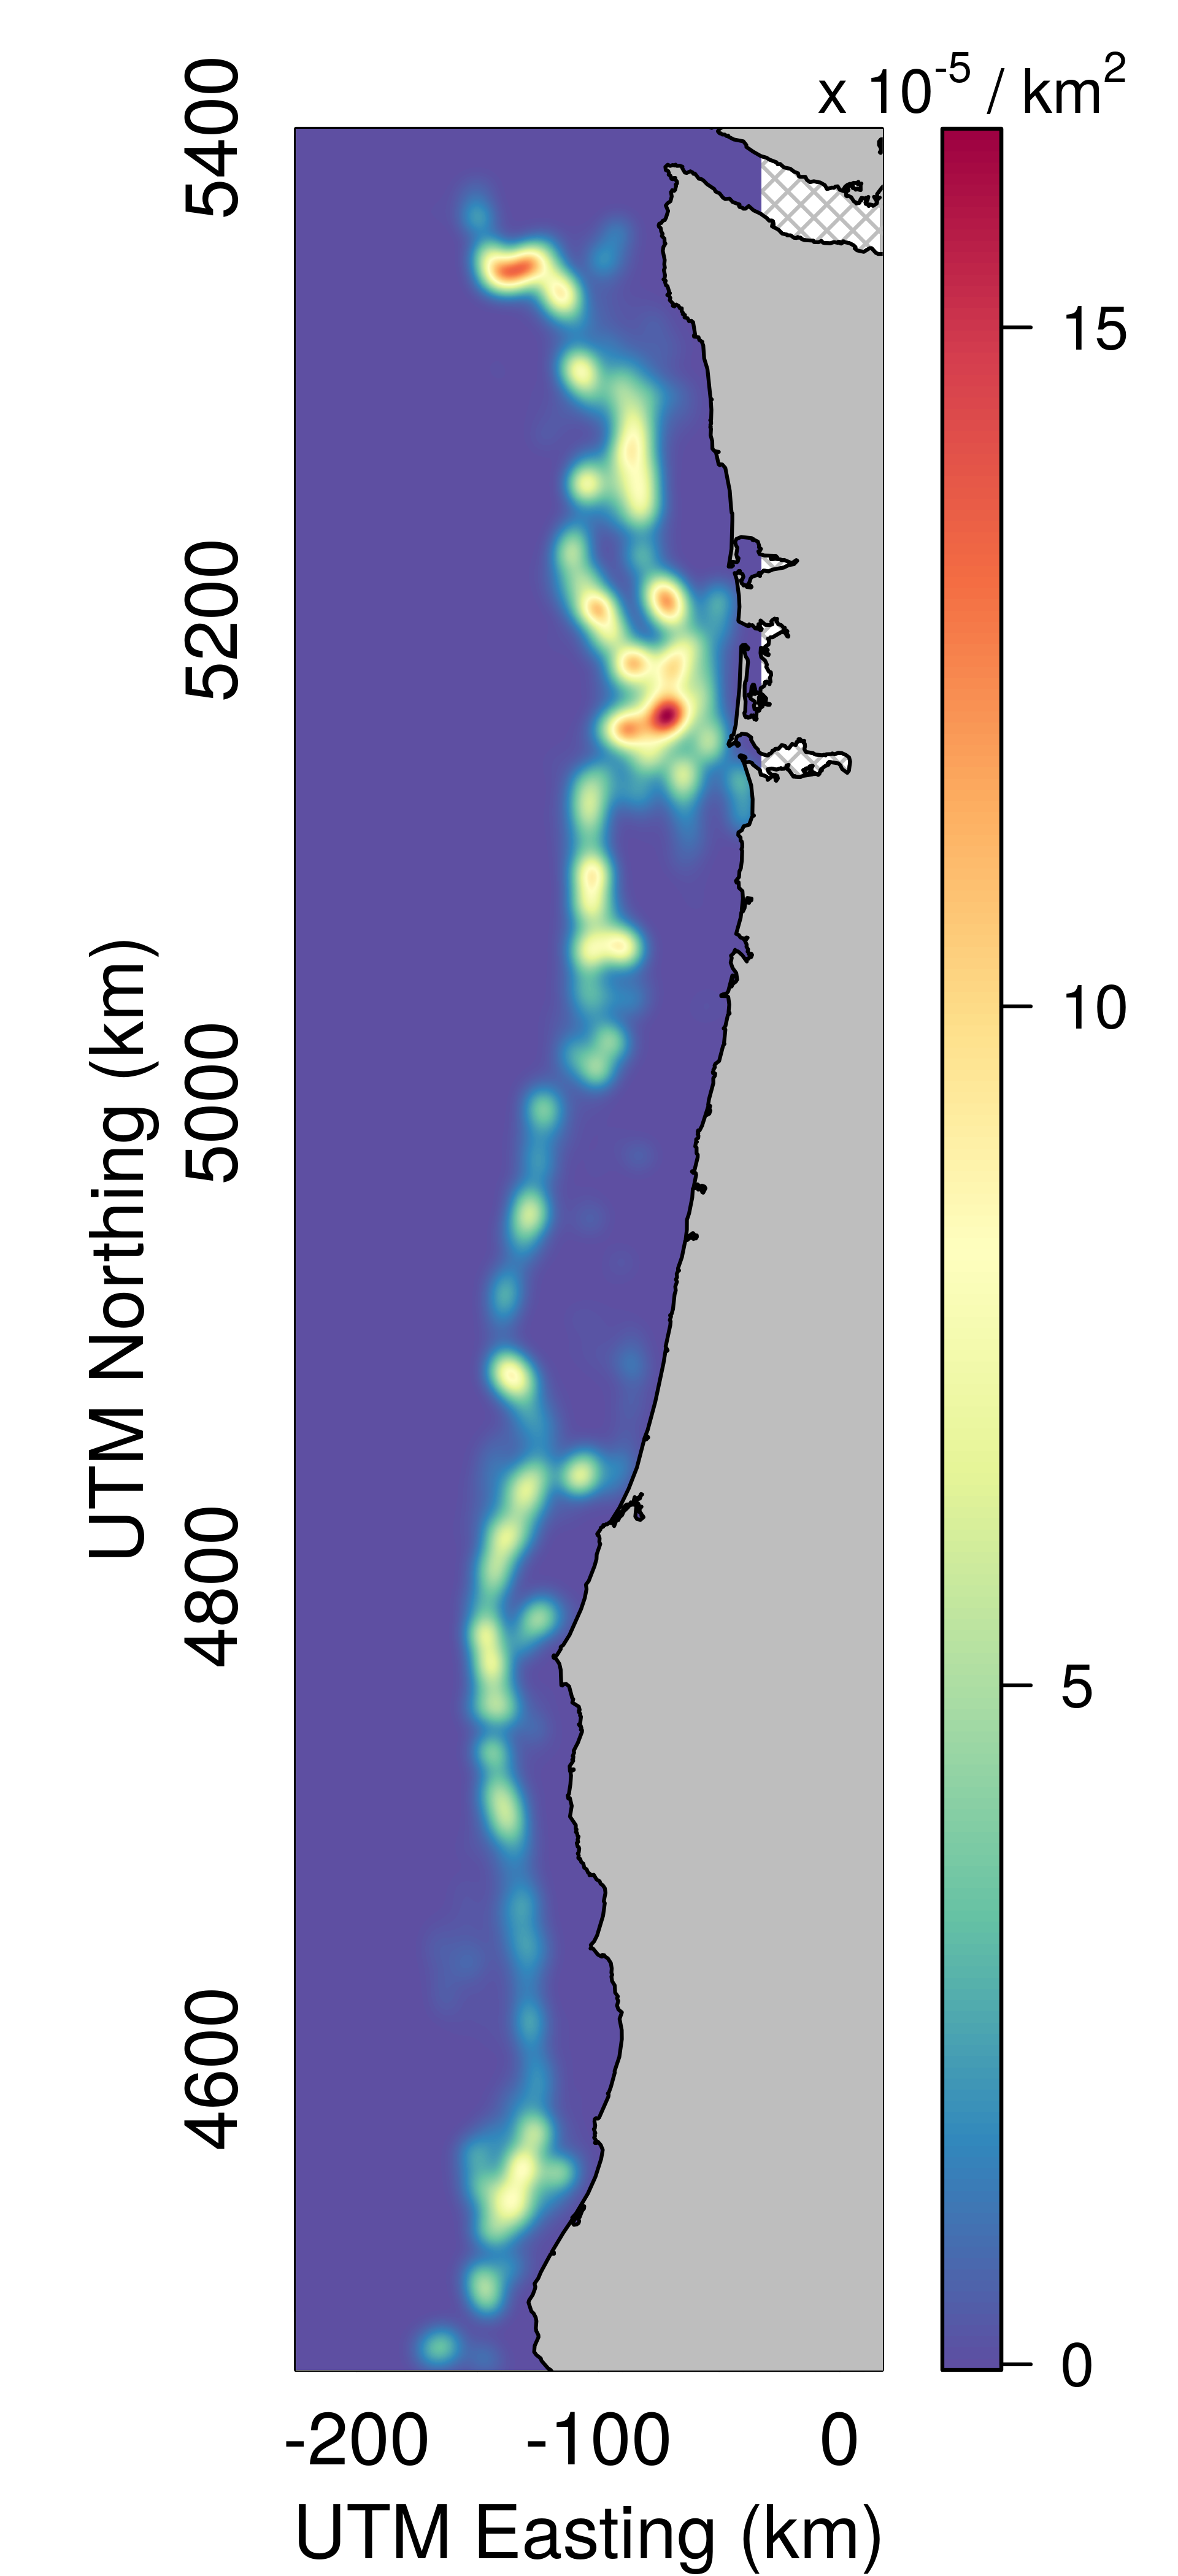
\includegraphics[width=2.5in]{../figures/fig1_effort_density/fig1_effort_density} 

}

\caption{Fishing effort density in the West Coast groundfish trawl fishery from 2011 to 2015 in the area north of Cape Falcon, Oregon (45.77° N). The West Coast Groundfish Observer Program monitored and collected data from 35,440 hauls from all (100\%) of the 4,007 trips. Fishing effort was smoothed using a bivariate kernel density estimate ('bkde2D' function in R package 'KernSmooth') to ensure that fishing locations were anonymized.}\label{fig:effort}
\end{figure}

\pagebreak

\begin{figure}

{\centering 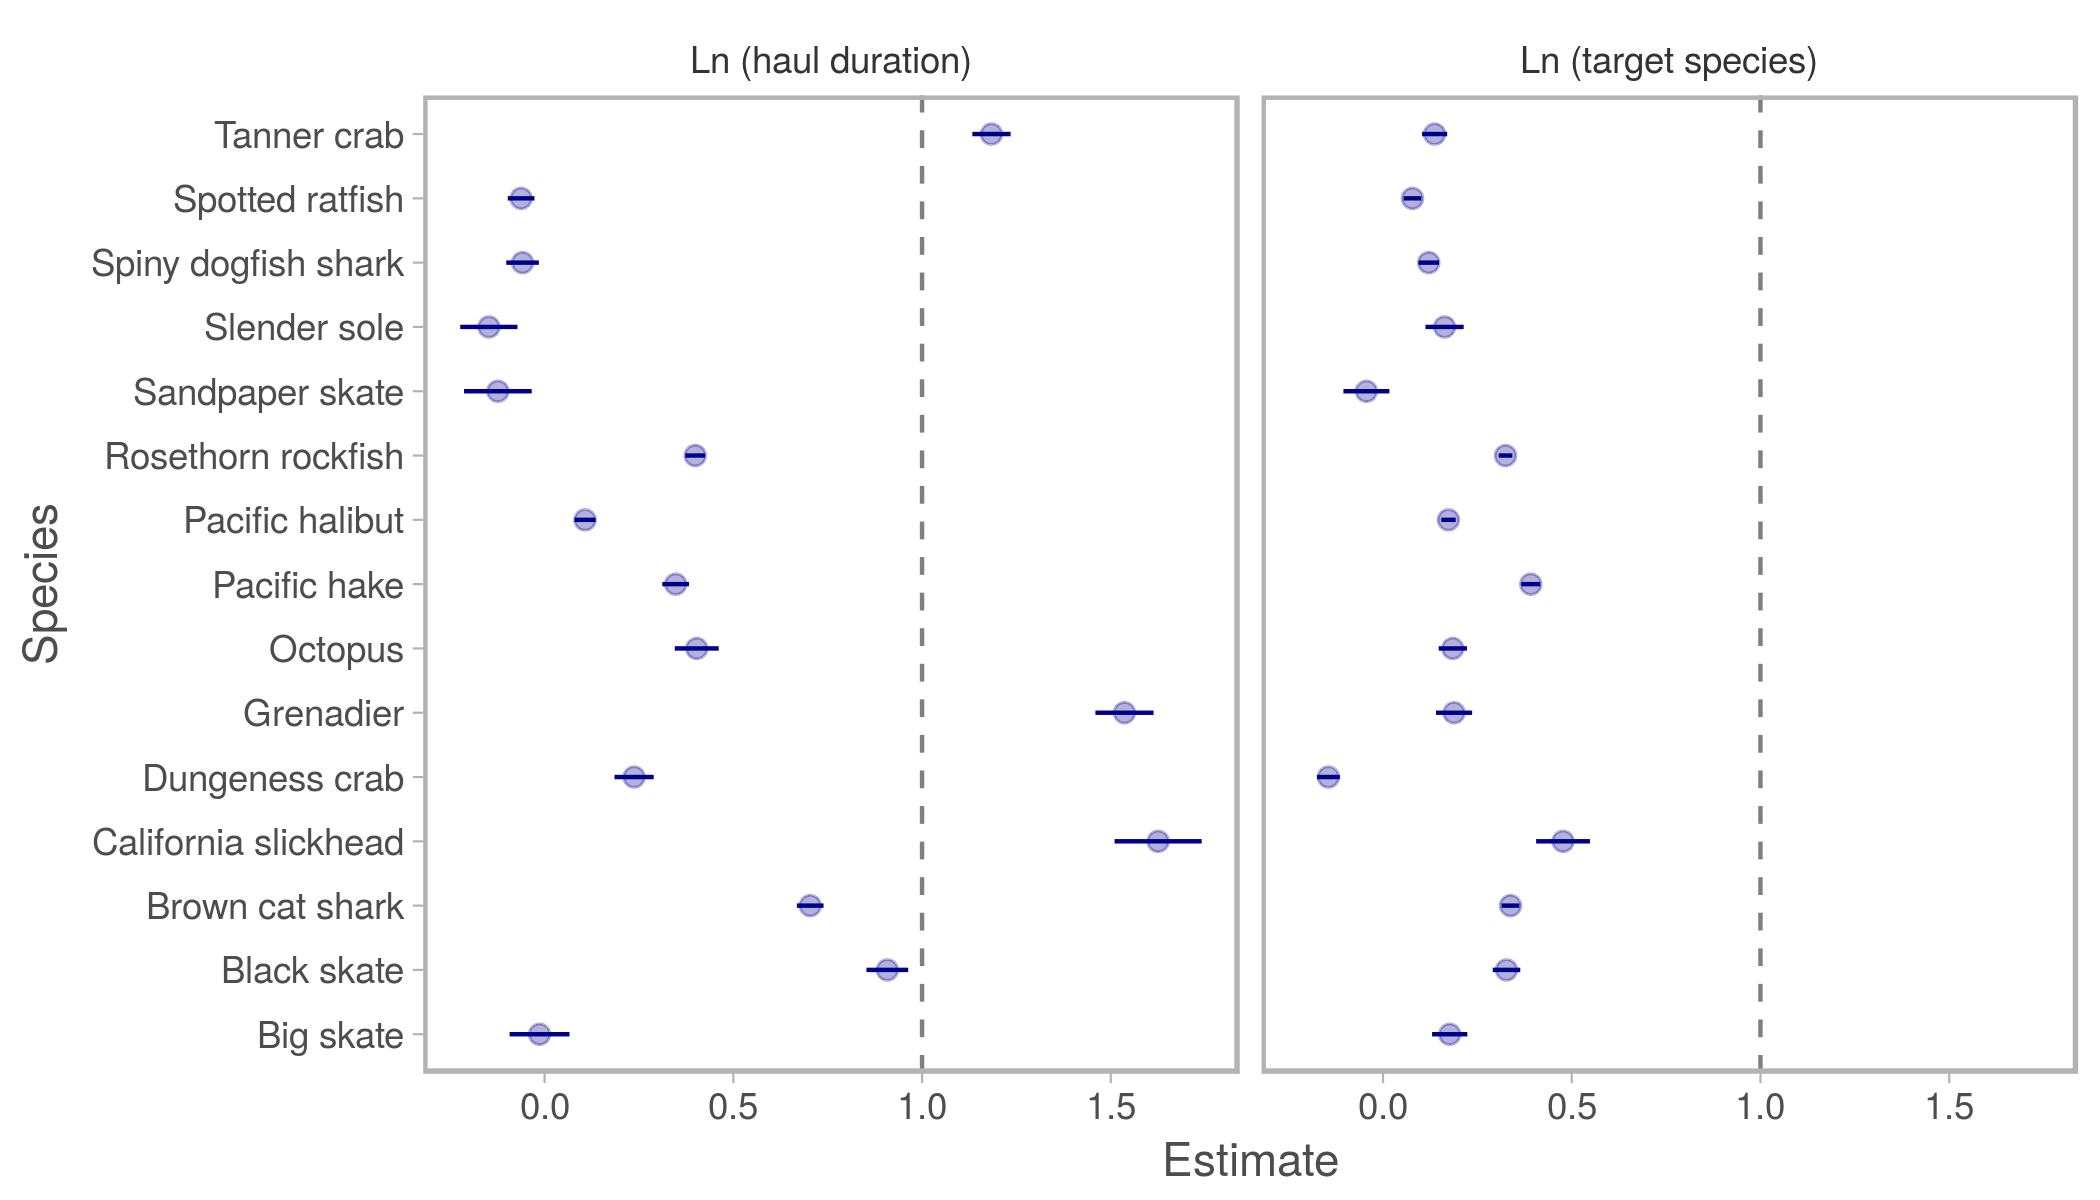
\includegraphics[width=6in]{../figures/fig2_effort_bycatch/fig2_effort_bycatch_caterpillar} 

}

\caption{Estimated relationships between fishing effort, defined as haul duration (hours, left panel) or catch of target species (kg, right panel), and bycatch for 15 species analyzed in the West Coast groundfish trawl fishery. The slope terms, $\beta$, of log-log linear models are exponents of an assumed power law fit to each species, $\text{Bycatch} = \alpha \text{Effort}^{\beta}$, with 95\% CIs shown for each estimate. Most $\beta$ are much less than 1 (left of dashed line), indicating the relationship between bycatch and effort is either weak or less-than-linear. Data ($n = 35,440$) consist of observed hauls from the West Coast Groundfish Observer Program recorded from 2011 to 2015 in the area north of Cape Falcon, Oregon (45.77° N).}\label{fig:effort-bycatch-slopes}
\end{figure}

\pagebreak

\begin{figure}

{\centering 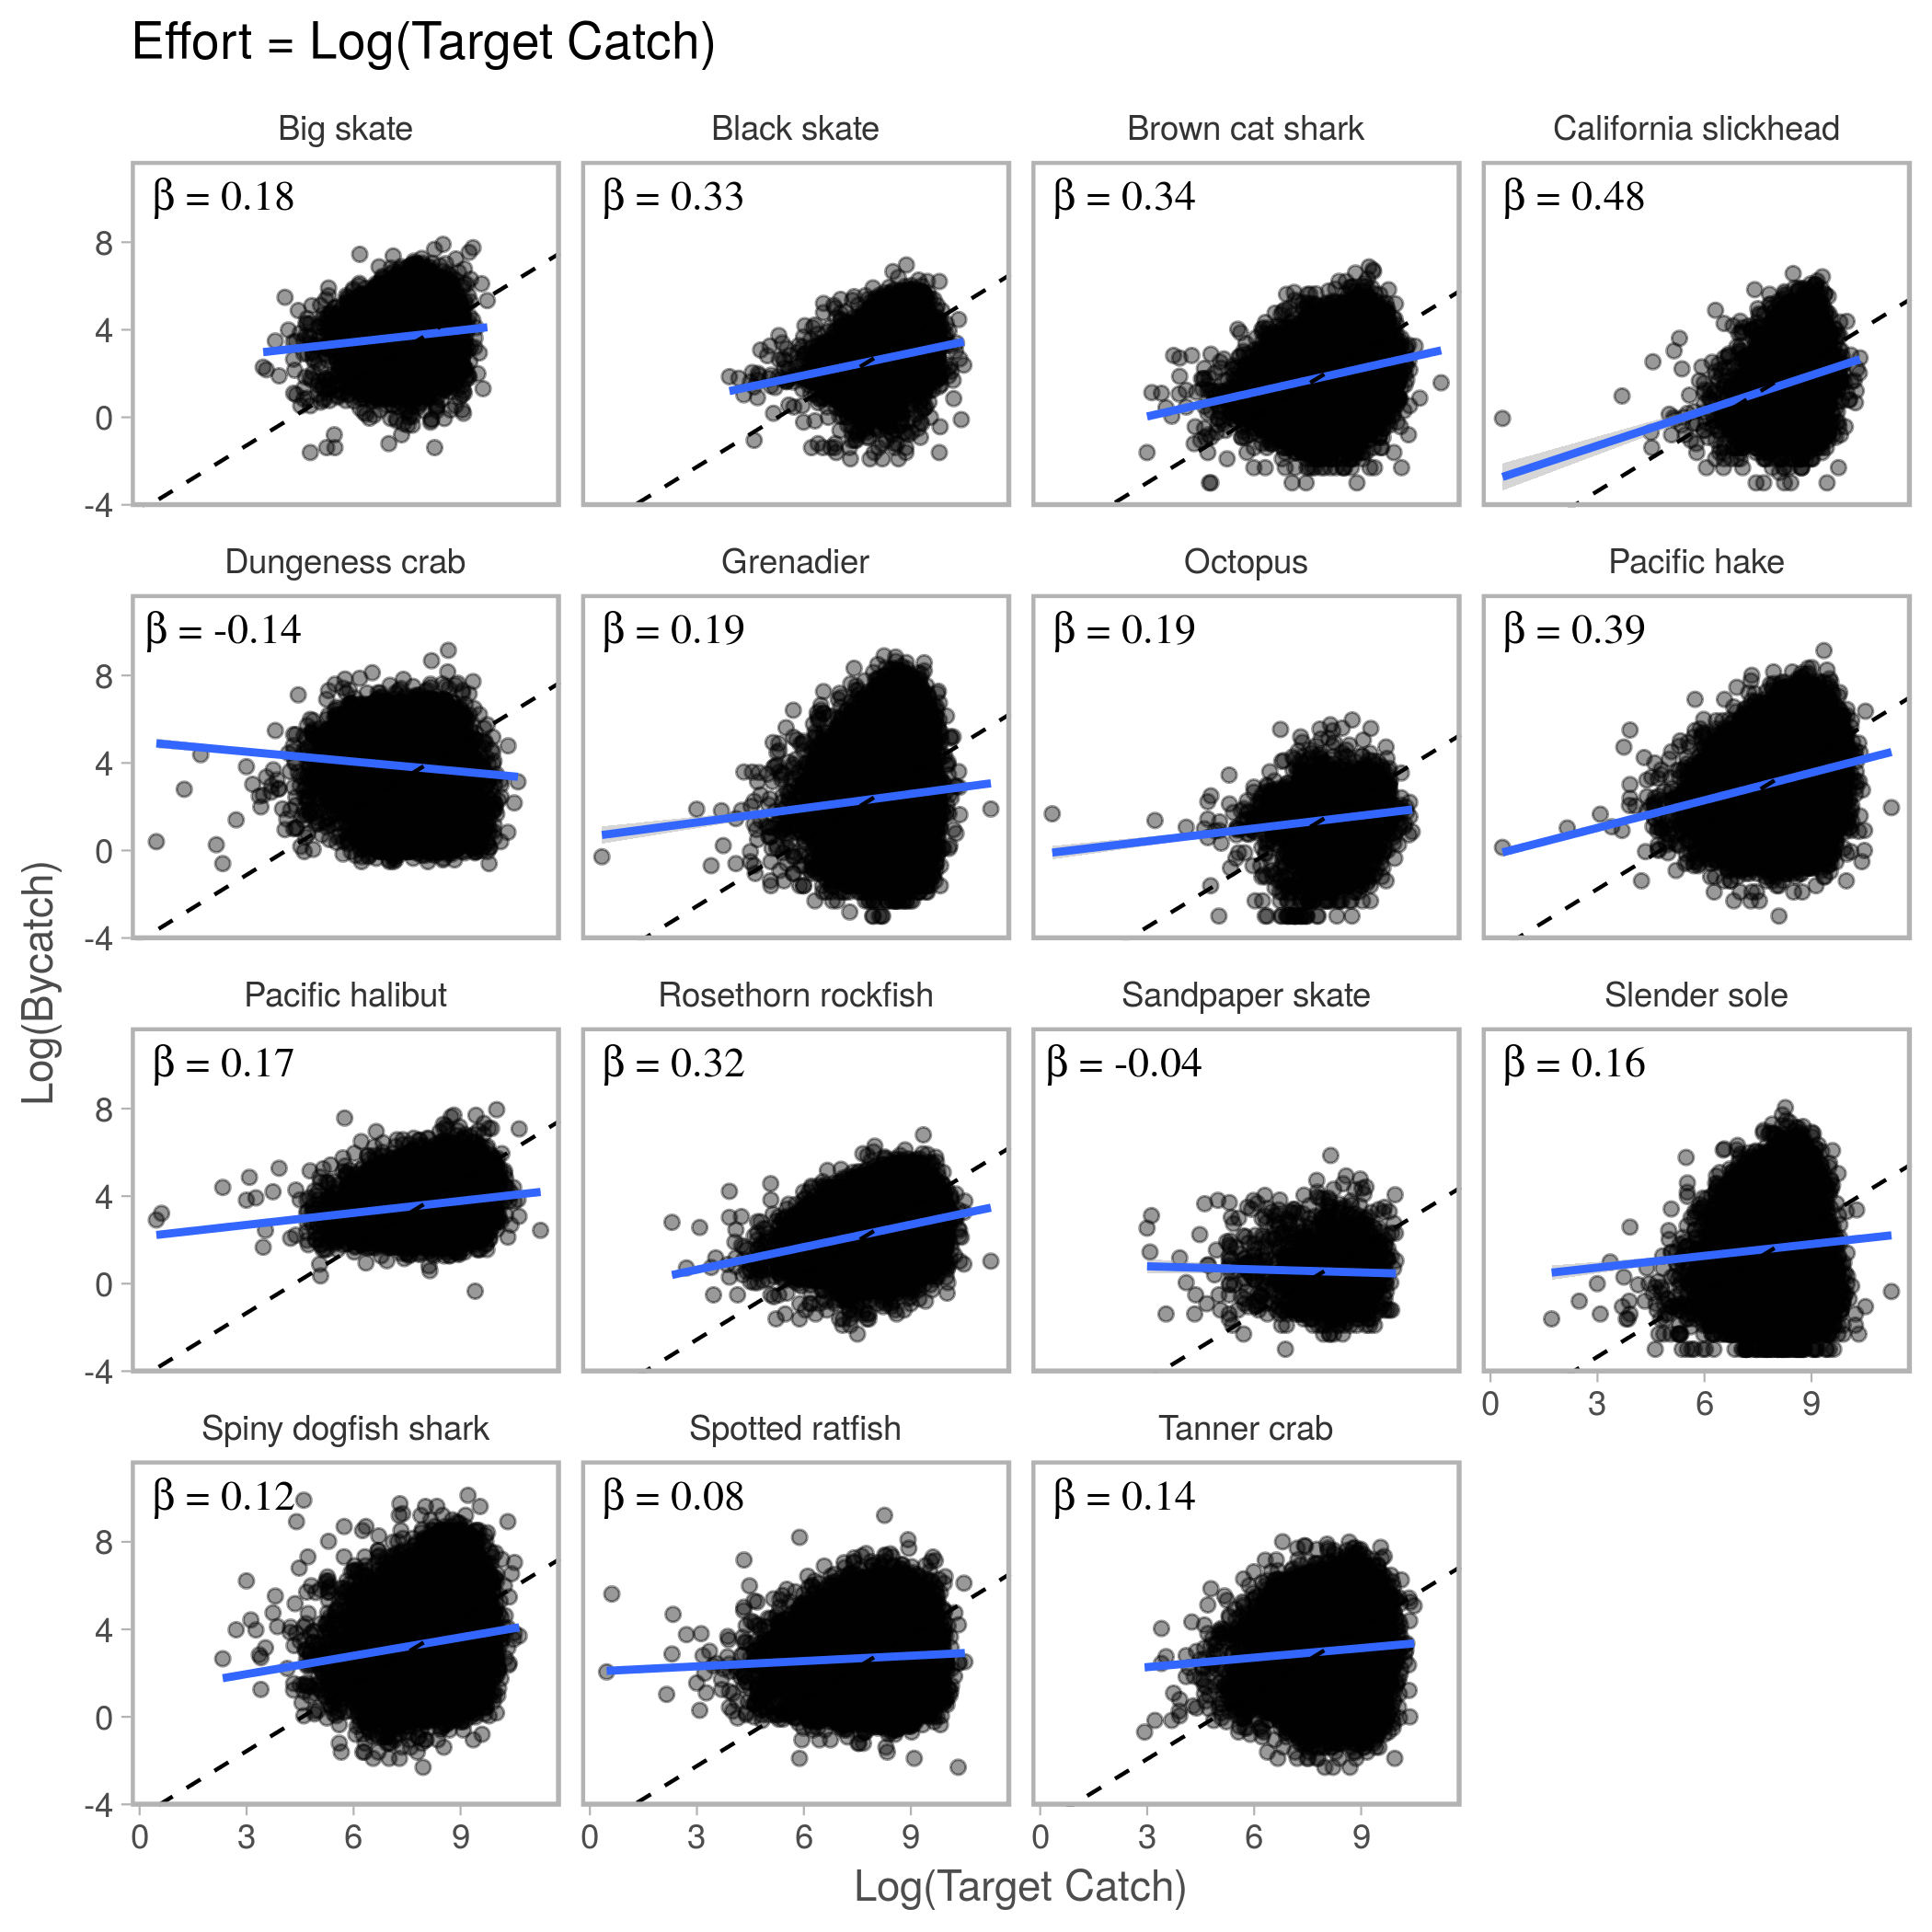
\includegraphics[width=6in]{../figures/fig2_effort_bycatch/fig2_effort_bycatch_target_nozeros} 

}

\caption{Relationship between fishing effort (catch of target species in kg) and bycatch (kg) of 15 selected species in the West Coast groundfish trawl fishery. The slope terms, $\beta$, of log-log linear models are exponents of an assumed power law fit to each species, $\text{Bycatch} = \alpha \text{Effort}^{\beta}$. All $\beta$ are much less than 1, indicating the relationship between Bycatch and Effort is either weak or less-than-linear. Each data point ($n = 35,440$) is an observed haul from the West Coast Groundfish Observer Program recorded from 2011 to 2015 in the area north of Cape Falcon, Oregon (45.77° N).}\label{fig:effort-bycatch}
\end{figure}

\pagebreak

\begin{figure}

{\centering 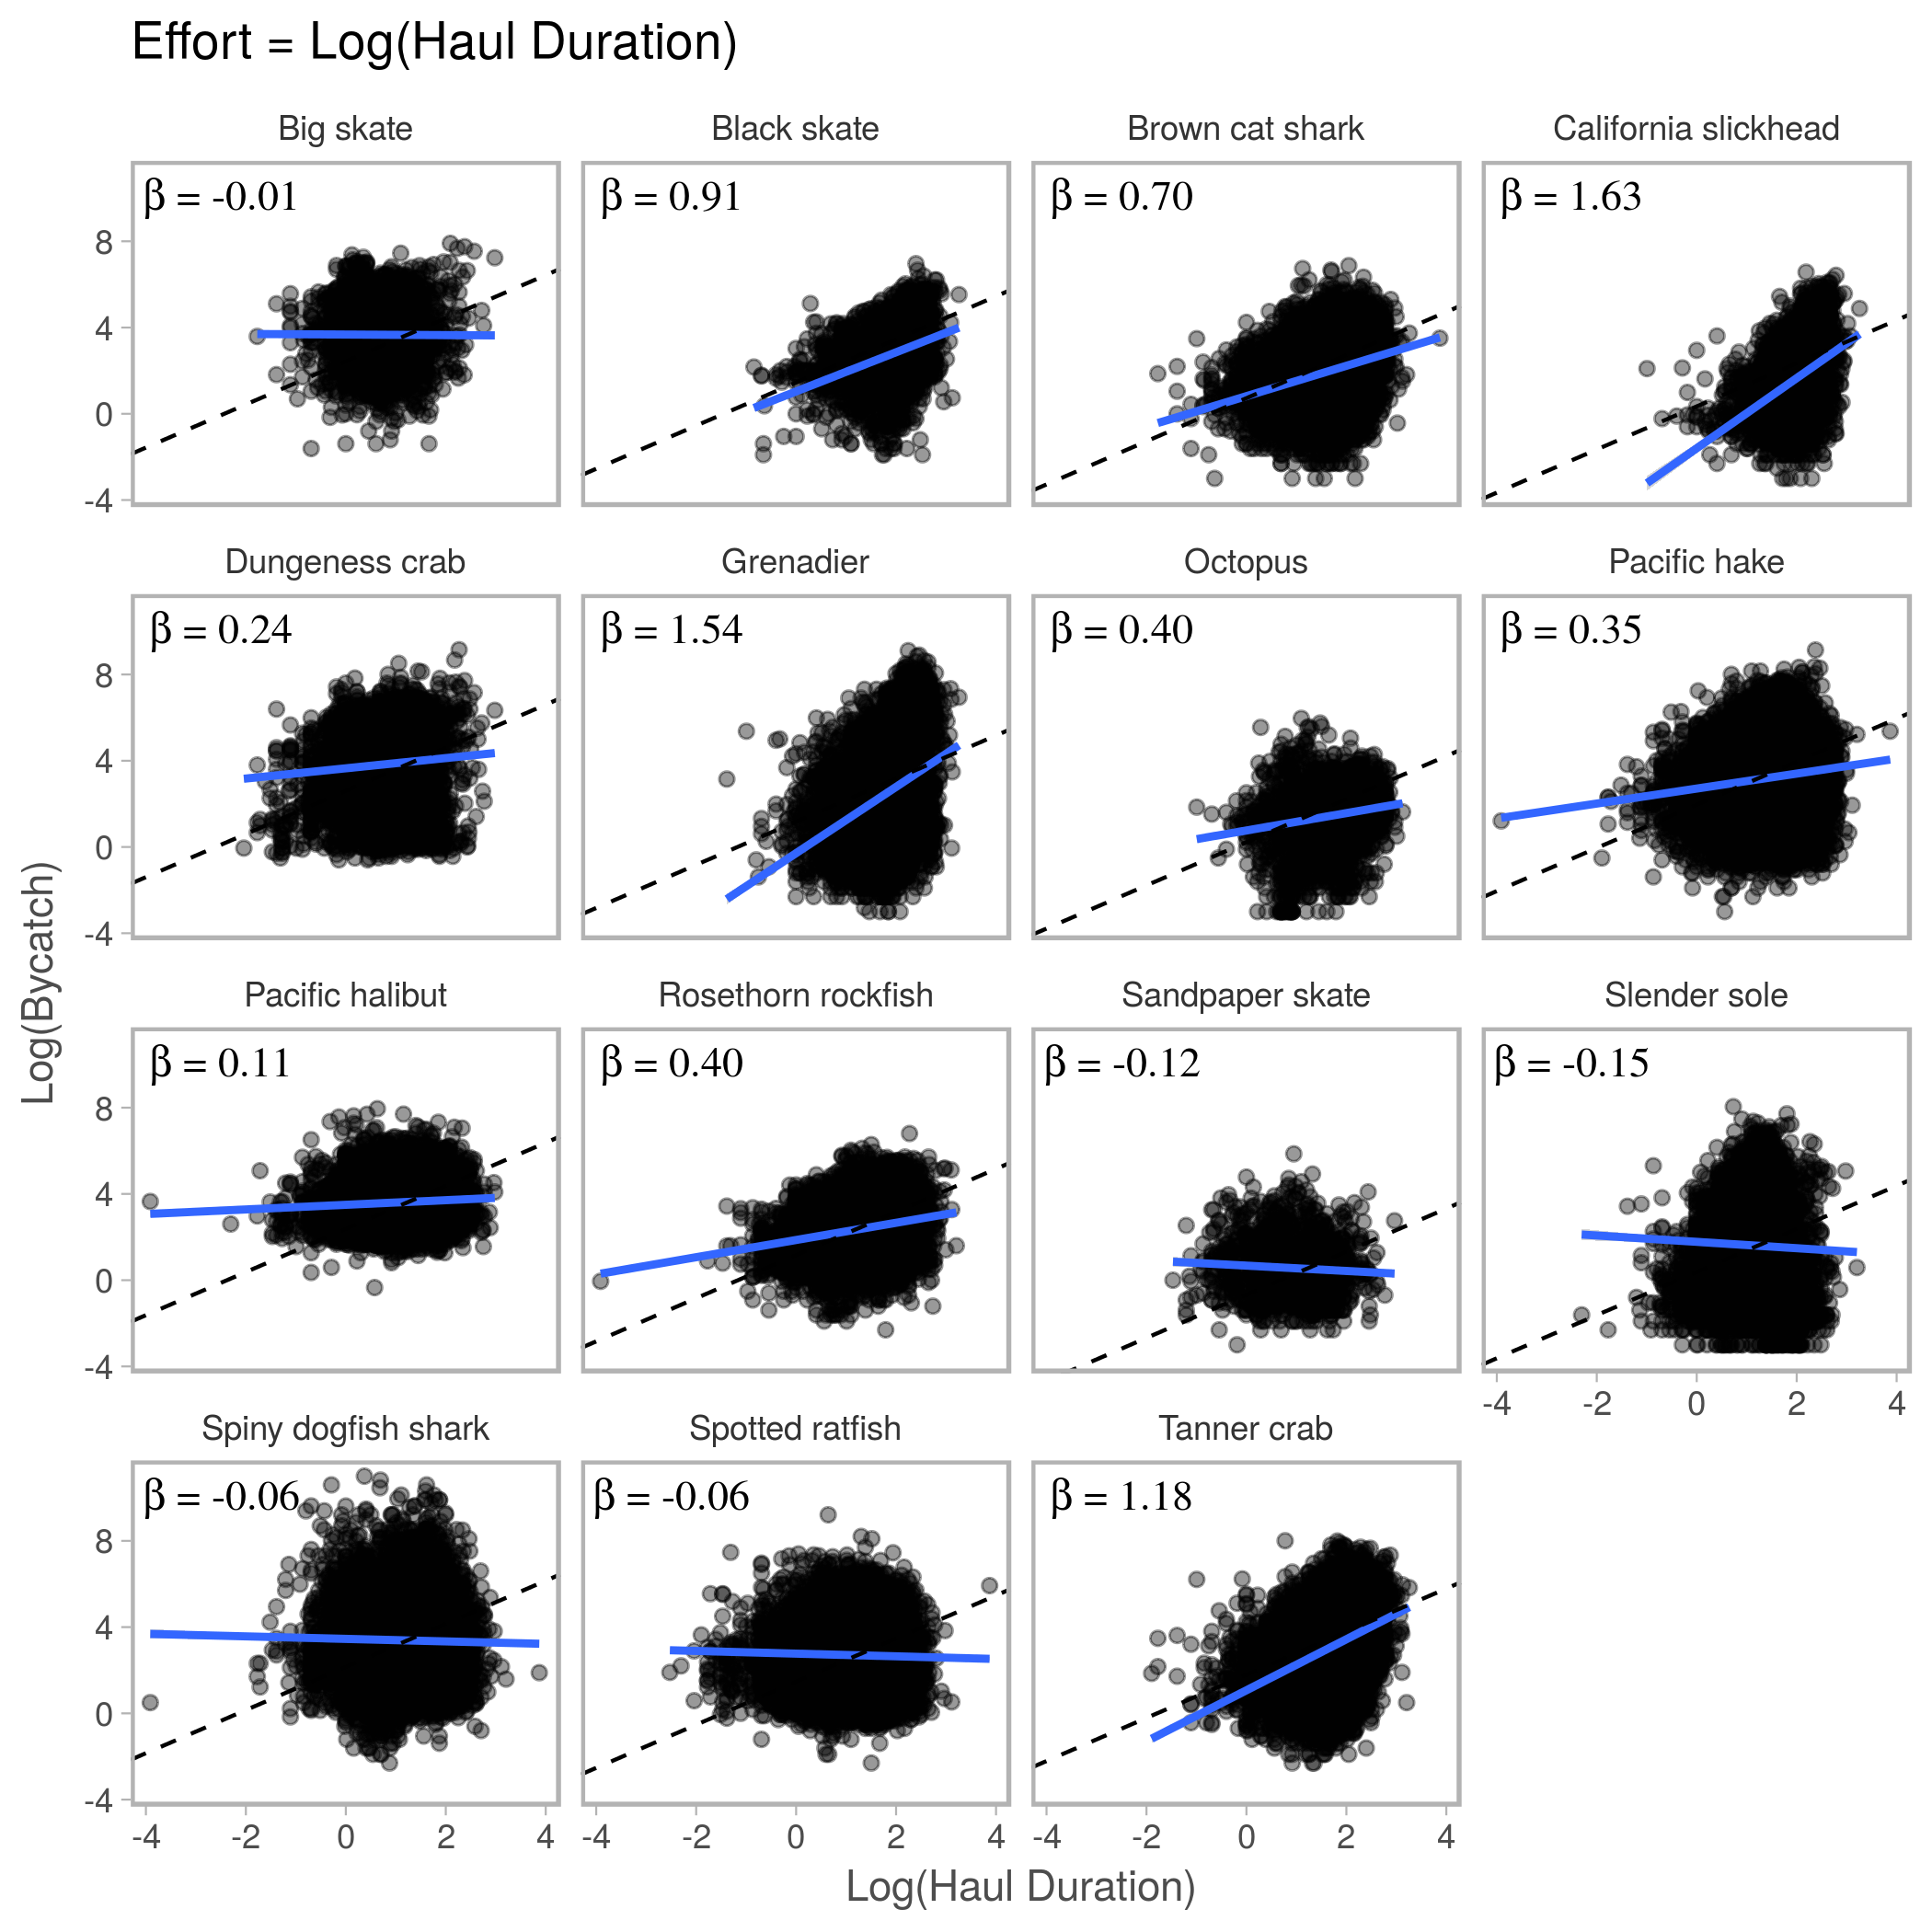
\includegraphics[width=6in]{../figures/fig2_effort_bycatch/fig2_effort_bycatch_hauldur} 

}

\caption{Estimated relationships between fishing effort (target catch in kg, haul duration in hours) and bycatch (kg) for 15 species analyzed in the West Coast groundfish trawl fishery. The slope terms, $\beta$, of log-log linear models are exponents of an assumed power law fit to each species, $\text{Bycatch} = \alpha \text{Effort}^{\beta}$, with 95-percent CIs shown for each estimate. Most $\beta$ are much less than 1, indicating the relationship between bycatch and effort is either weak or not linear. Data ($n = 35,440$) consist of observed hauls from the West Coast Groundfish Observer Program recorded from 2011 to 2015 in the area north of Cape Falcon, Oregon (45.77° N).}\label{fig:effort-bycatch-2}
\end{figure}

\pagebreak

\begin{figure}

{\centering 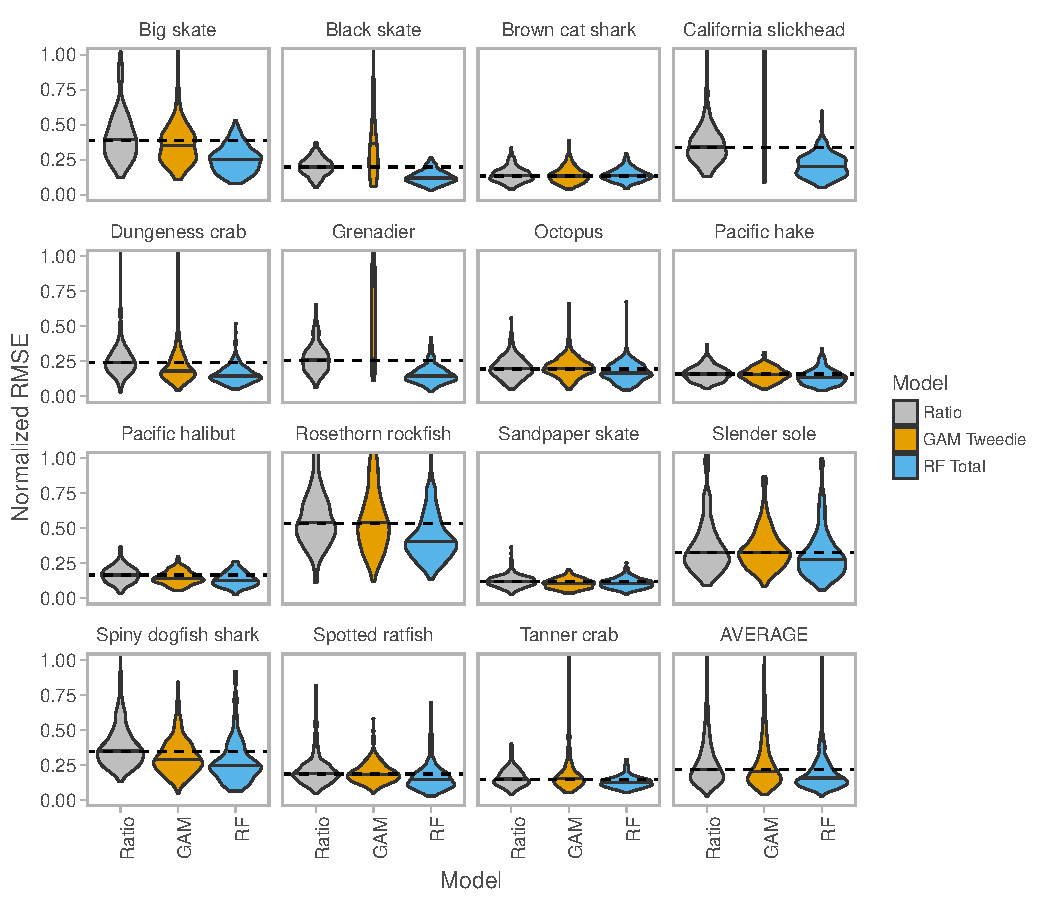
\includegraphics{bycatch_sim_paper_files/figure-latex/model-comparison-1} 

}

\caption{Predictive performance of the ratio estimator (status quo) and two spatial modeling frameworks: generalized additive model (GAM) and random forest (RF). We fit each model to 200 'training' datasets simulated with 20\% observer coverage, then predicted bycatch in unobserved hauls to calculate annual estimates of fleet-wide bycatch. We calculated model performance (RMSE) using the true, observed bycatch. For each species, the dashed line indicates the median RMSE for the ratio estimator, and solid lines indicate median RMSE for each model. The GAM-Tweedie had convergence issues for 3/15 species. RF-Total outperformed the ratio estimator for all species, and on average had 26\% lower RMSE (RF = 0.16, Ratio = 0.22).}\label{fig:model-comparison}
\end{figure}

\pagebreak

\begin{landscape}
\begin{figure}

{\centering 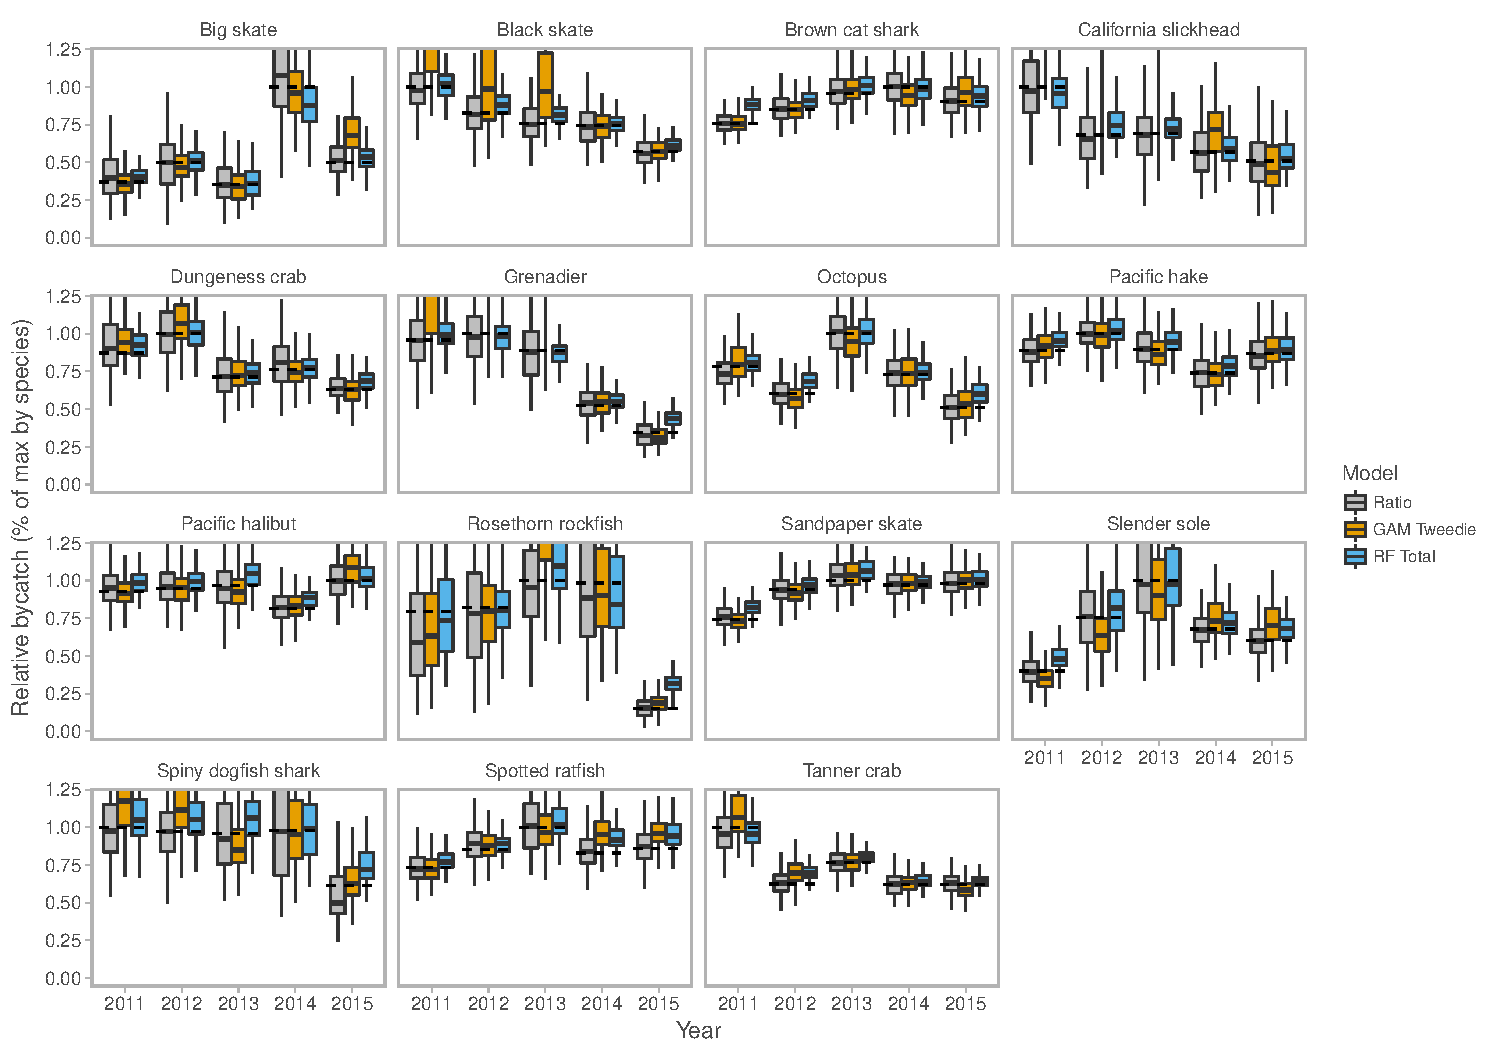
\includegraphics[width=10in]{bycatch_sim_paper_files/figure-latex/model-comparison-byyear-catch-1} 

}

\caption{Predictive performance of the ratio estimator (status quo) and two spatial modeling frameworks: generalized additive model (GAM) and random forests (RF). We fit each model to 200 'training' datasets simulated with 20\% observer coverage, then predicted bycatch in unobserved hauls to calculate annual estimates of fleet-wide bycatch. For each species and year, the dashed lines indicate the true observed bycatch.}\label{fig:model-comparison-byyear-catch}
\end{figure}
\end{landscape}

\pagebreak

\begin{figure}

{\centering 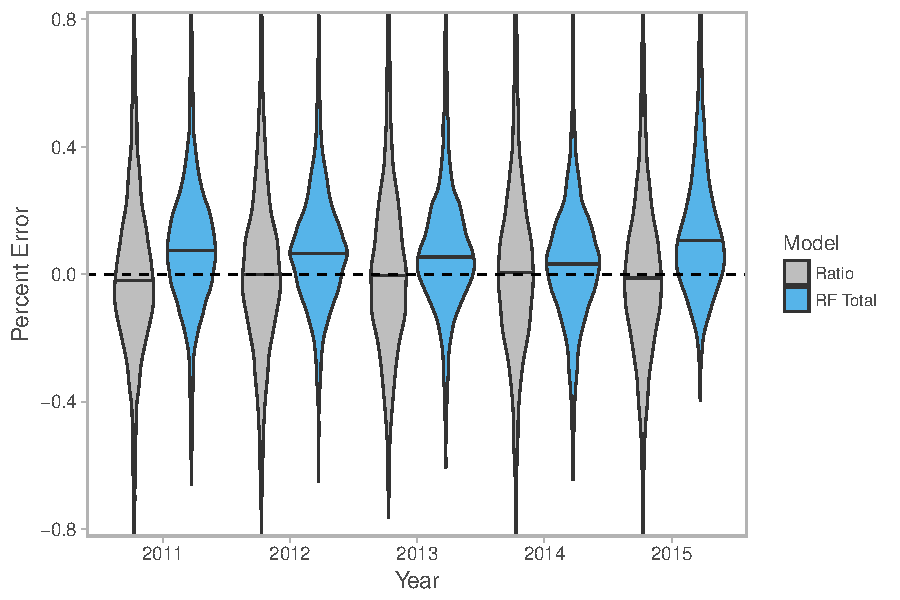
\includegraphics[width=6in]{bycatch_sim_paper_files/figure-latex/model-comparison-byyear-1} 

}

\caption{Percent error of annual bycatch predictions using the ratio estimator (status quo) and random forests (RF), averaged across 15 species in the West Coast groundfish trawl fishery. Averaged across species, RF-Total was more precise than the ratio estimator (median absolute percent error: RF = 0.118, Ratio = 0.155), but with slight positive bias (median percent error = 0.068). Median percent error (bias) of the ratio estimator was very slightly negative (-0.011). We fit each model to 200 'training' datasets simulated with 20\% observer coverage, then predicted bycatch in unobserved hauls to calculate annual estimates of fleet-wide bycatch for each species. Percent error was calculated using the true, observed bycatch.}\label{fig:model-comparison-byyear}
\end{figure}

\pagebreak

\begin{figure}

{\centering 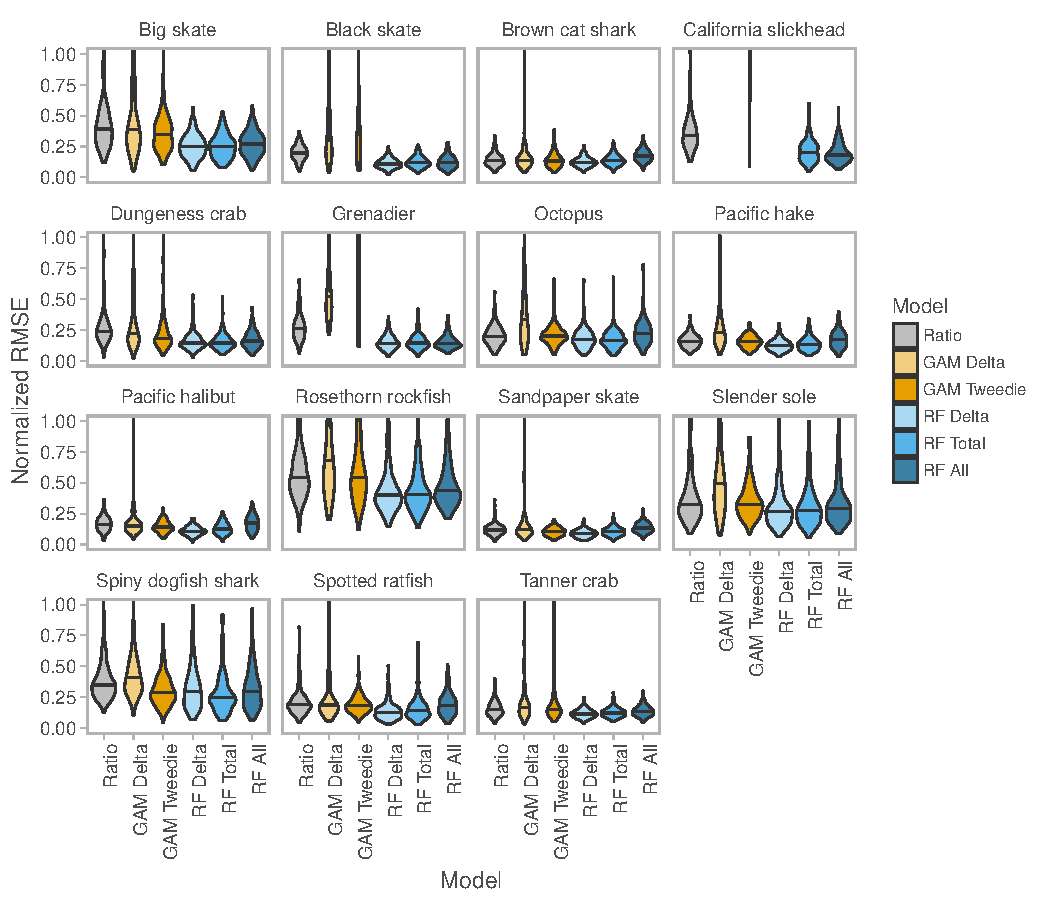
\includegraphics[width=7in]{bycatch_sim_paper_files/figure-latex/model-comparison-delta-1} 

}

\caption{Predictive performance of the ratio estimator (status quo) and two spatial modeling frameworks: generalized additive model (GAM) and random forests (RF). We fit each model to 200 'training' datasets simulated with 20\% observer coverage, then predicted bycatch in unobserved hauls to calculate annual estimates of fleet-wide bycatch. For each species, the dashed line indicates the median RMSE for the ratio estimator, and solid lines indicate median RMSE for each model. For both GAMs and RFs, the non-delta models outperformed the delta models.}\label{fig:model-comparison-delta}
\end{figure}

\pagebreak

\begin{figure}

{\centering 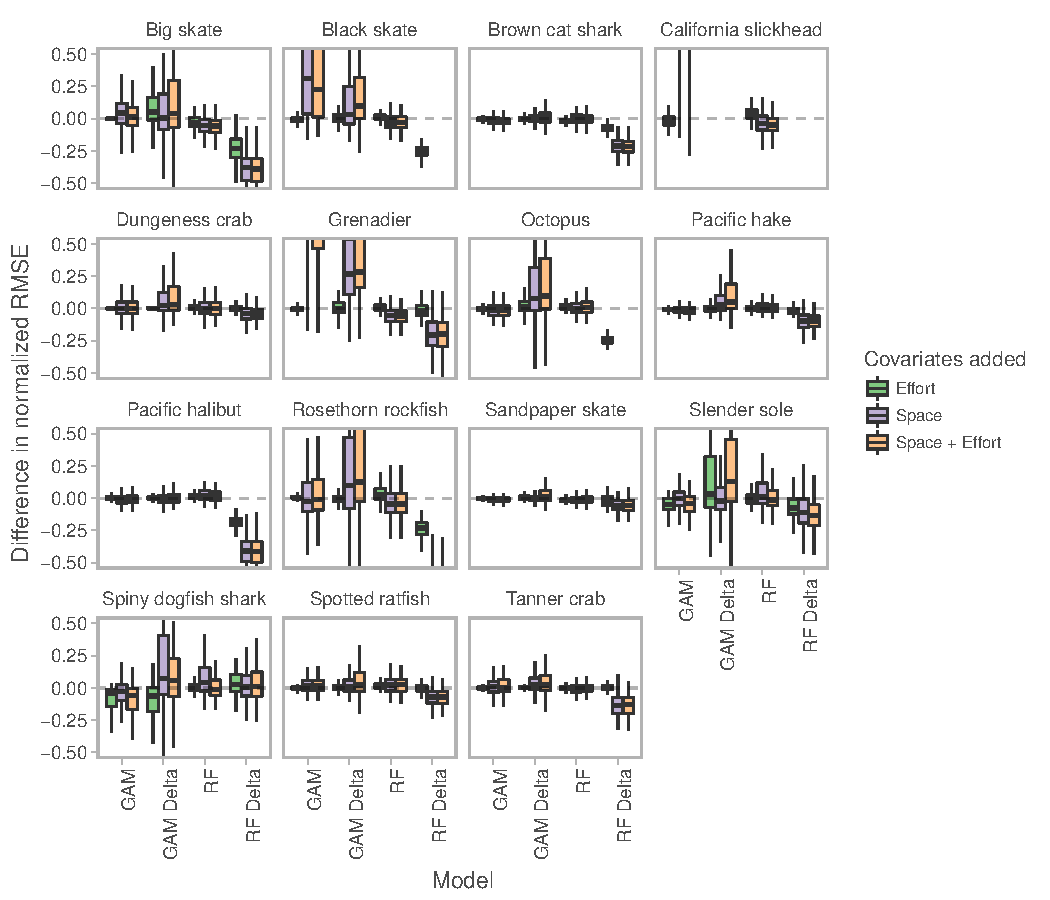
\includegraphics[width=7in]{bycatch_sim_paper_files/figure-latex/covariate-effects-1} 

}

\caption{Change in predictive performance (normalized RMSE) when adding fishing effort and spatial location as covariates in each model. For many species, adding space to the GAM-Delta and GAM-Tweedie models led to worse predictions (positive change in RMSE, above dashed line). On the other hand, adding space to the RF-Delta model consistently improved predictions (negative change in RMSE, below dashed line). For RF-Total, including space had either slightly improved predictions or had no effect. Adding effort had little effect for nearly all species and models, and never had a larger effect than adding space.}\label{fig:covariate-effects}
\end{figure}

\pagebreak

\begin{figure}

{\centering 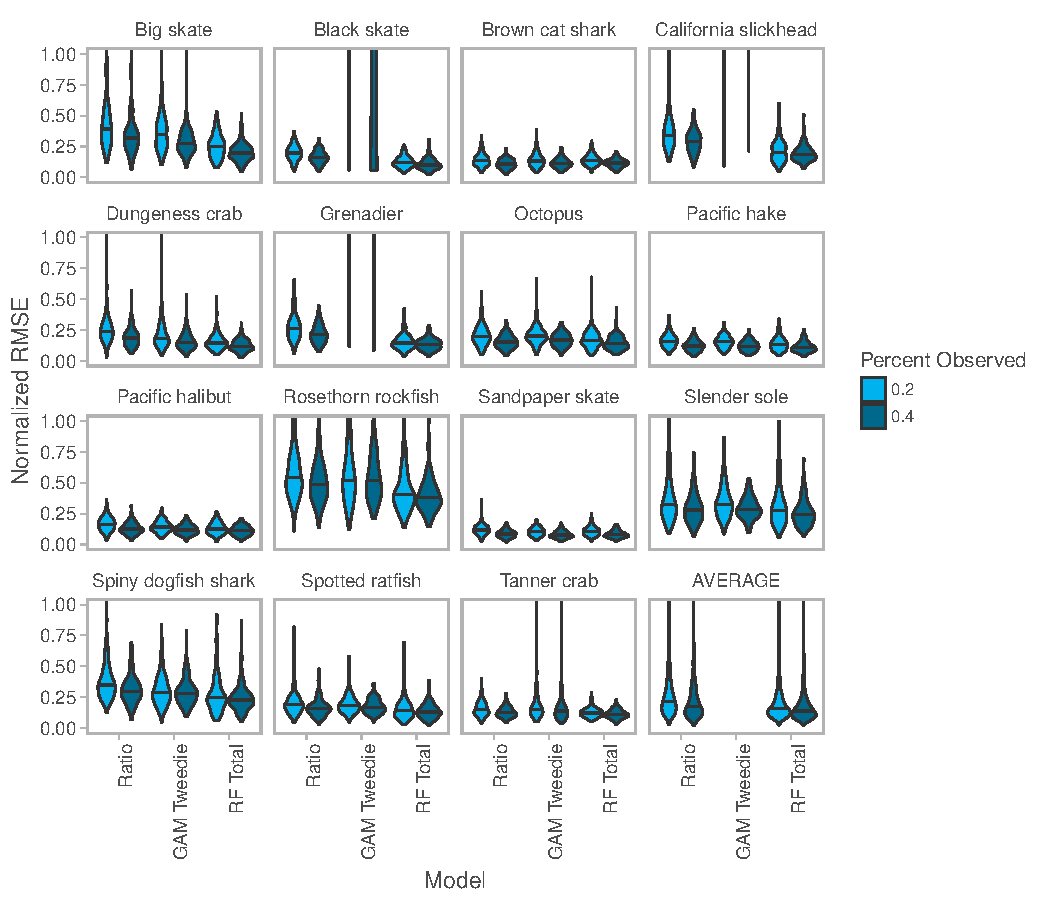
\includegraphics[width=7in]{bycatch_sim_paper_files/figure-latex/coverage-effects-1} 

}

\caption{Predictive performance (normalized RMSE) for different levels of simulated observer coverage. Averaged across species, RF-Total had lower median RMSE than the ratio estimator, even at half the observer coverage (RF-Total at 20\%: 0.155, Ratio at 40\%: 0.180). GAM-Tweedie failed to converge for 3/15 species.}\label{fig:coverage-effects}
\end{figure}

\pagebreak

\begin{figure}

{\centering 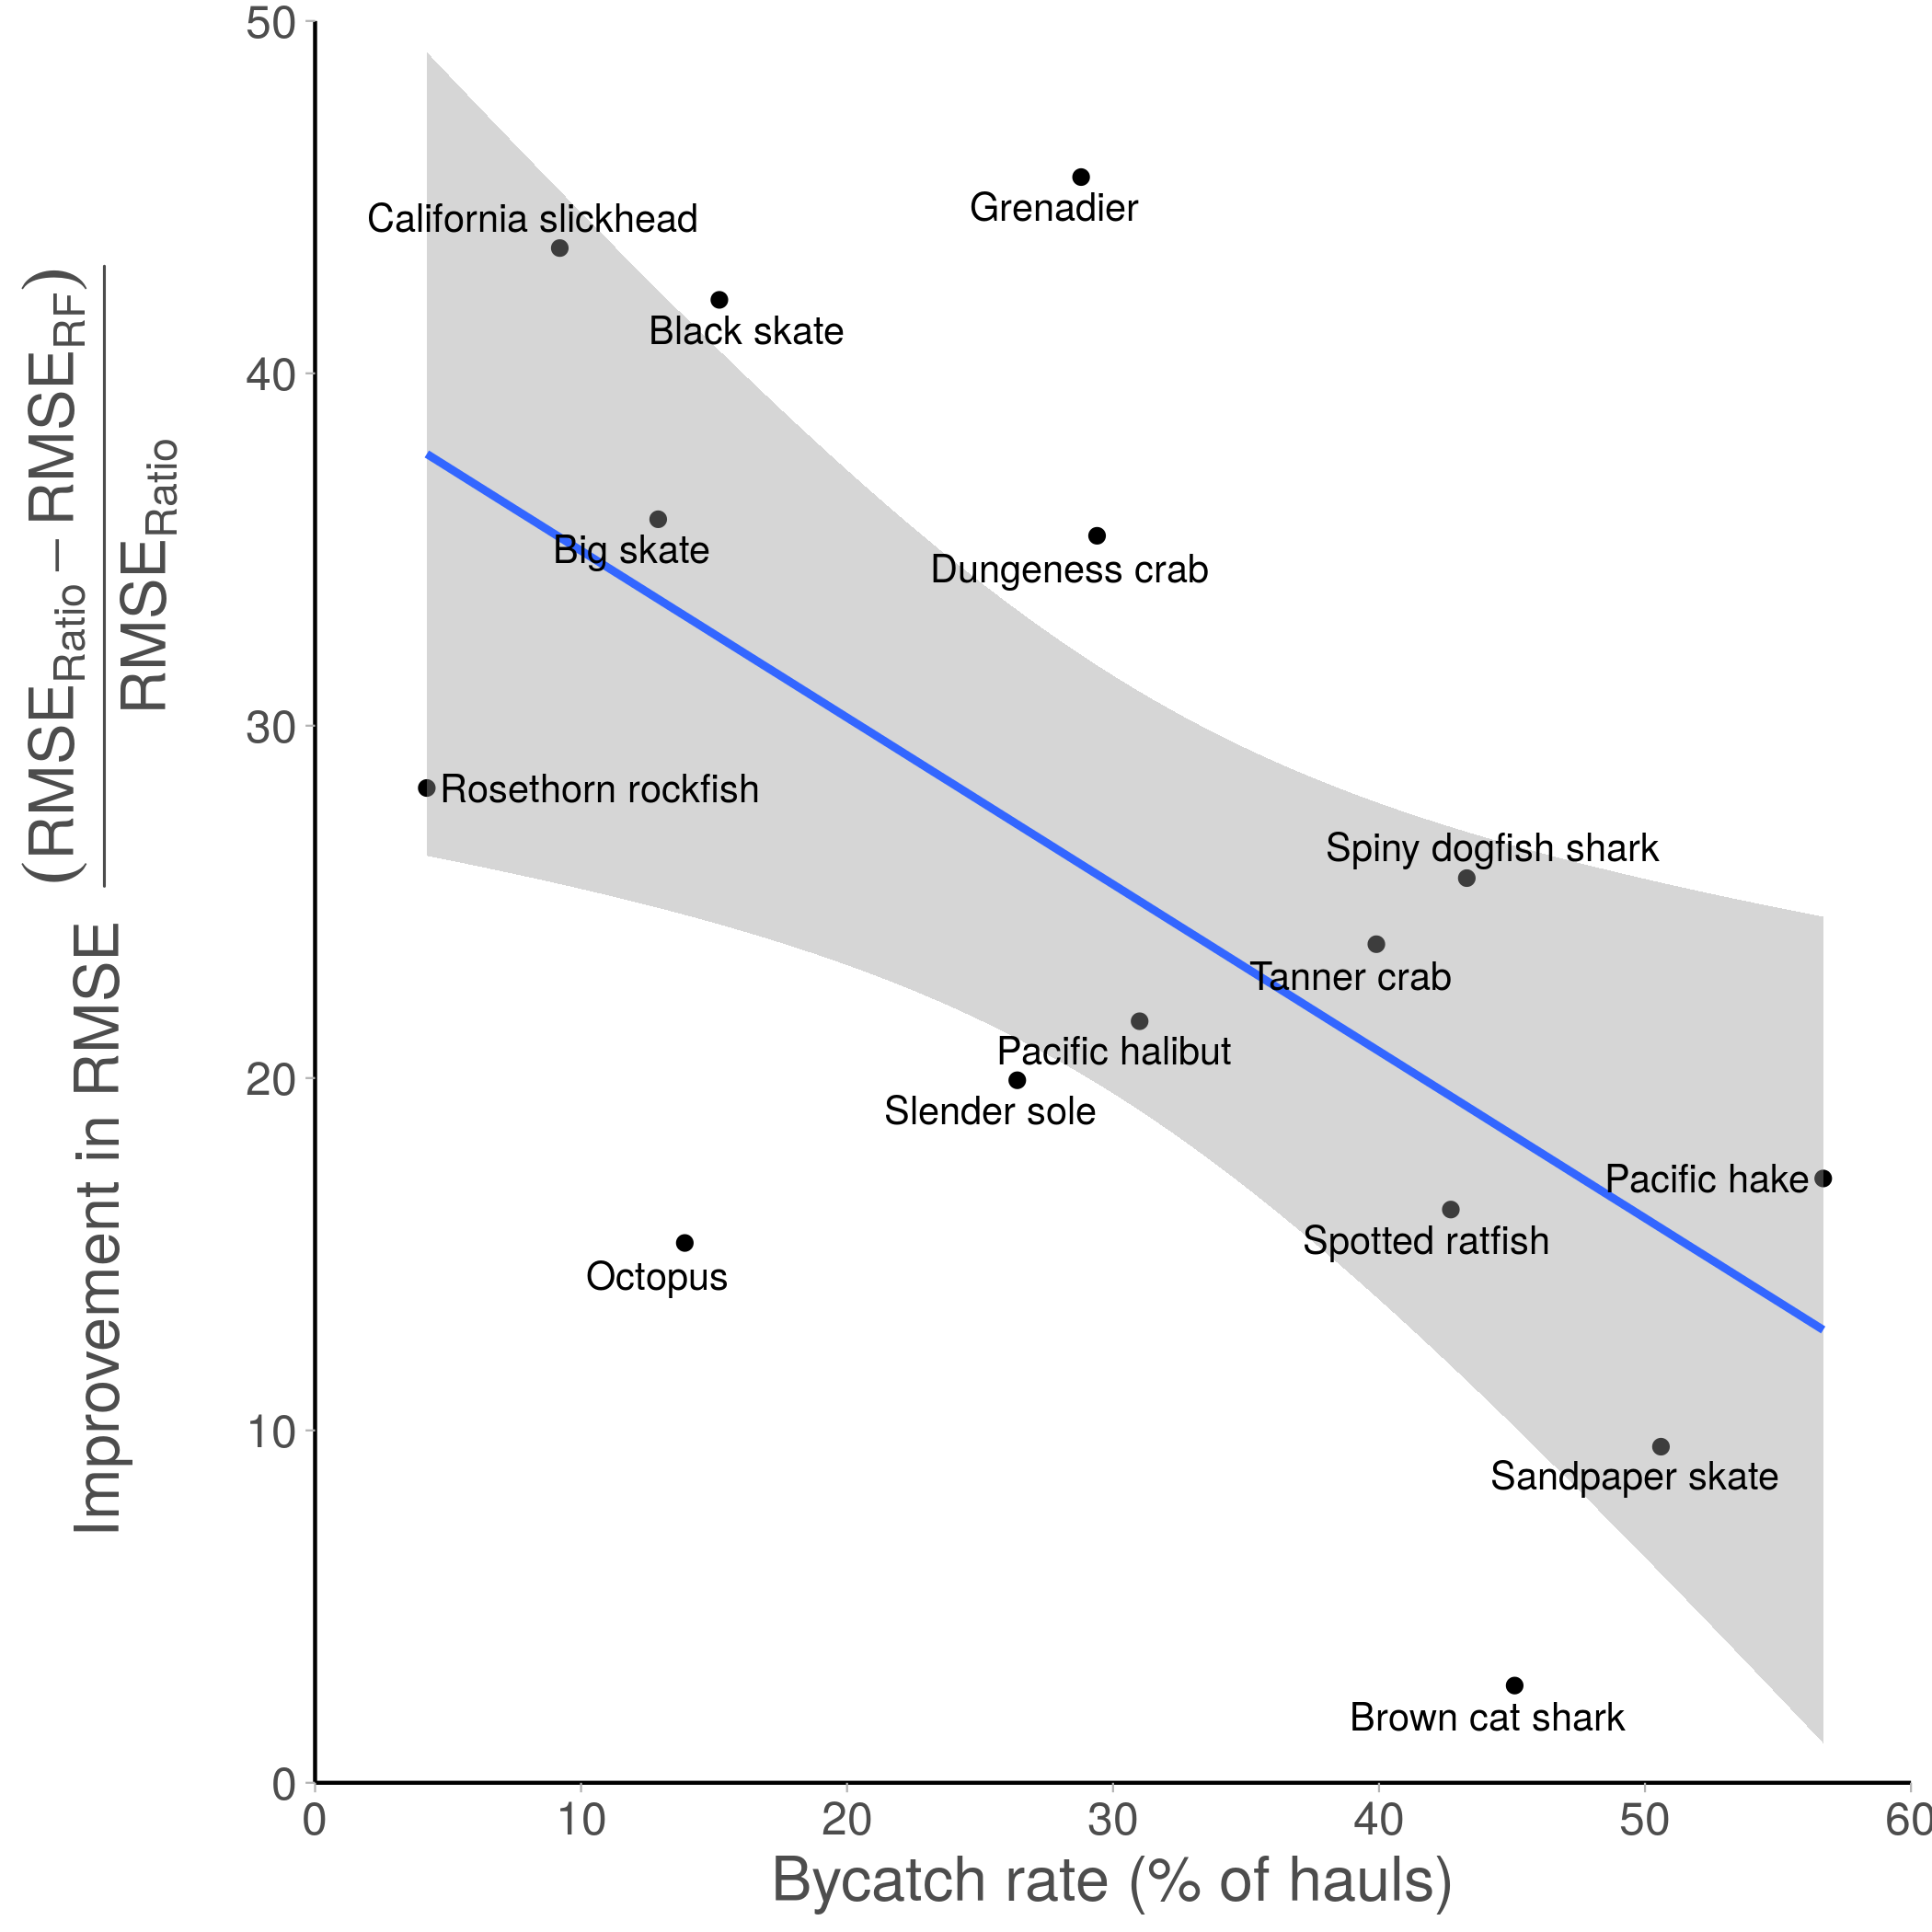
\includegraphics[width=6in]{../figures/supplement/fig10_bycatch_rate_rmse} 

}

\caption{RF reduction in prediction error compared to the ratio estimator, as a function of bycatch rate for 15 species in the U.S. West Coast groundfish trawl fishery. RF improved on the ratio estimator for all species (26\% lower RMSE on average), but this improvement was greater for species with lower bycatch rates (e.g. Rosethorn rockfish, California slickhead, Big skate, Black skate, Dungeness crab, Grenadier).}\label{fig:bycatch-rate-rmse}
\end{figure}

\pagebreak

\begin{figure}

{\centering 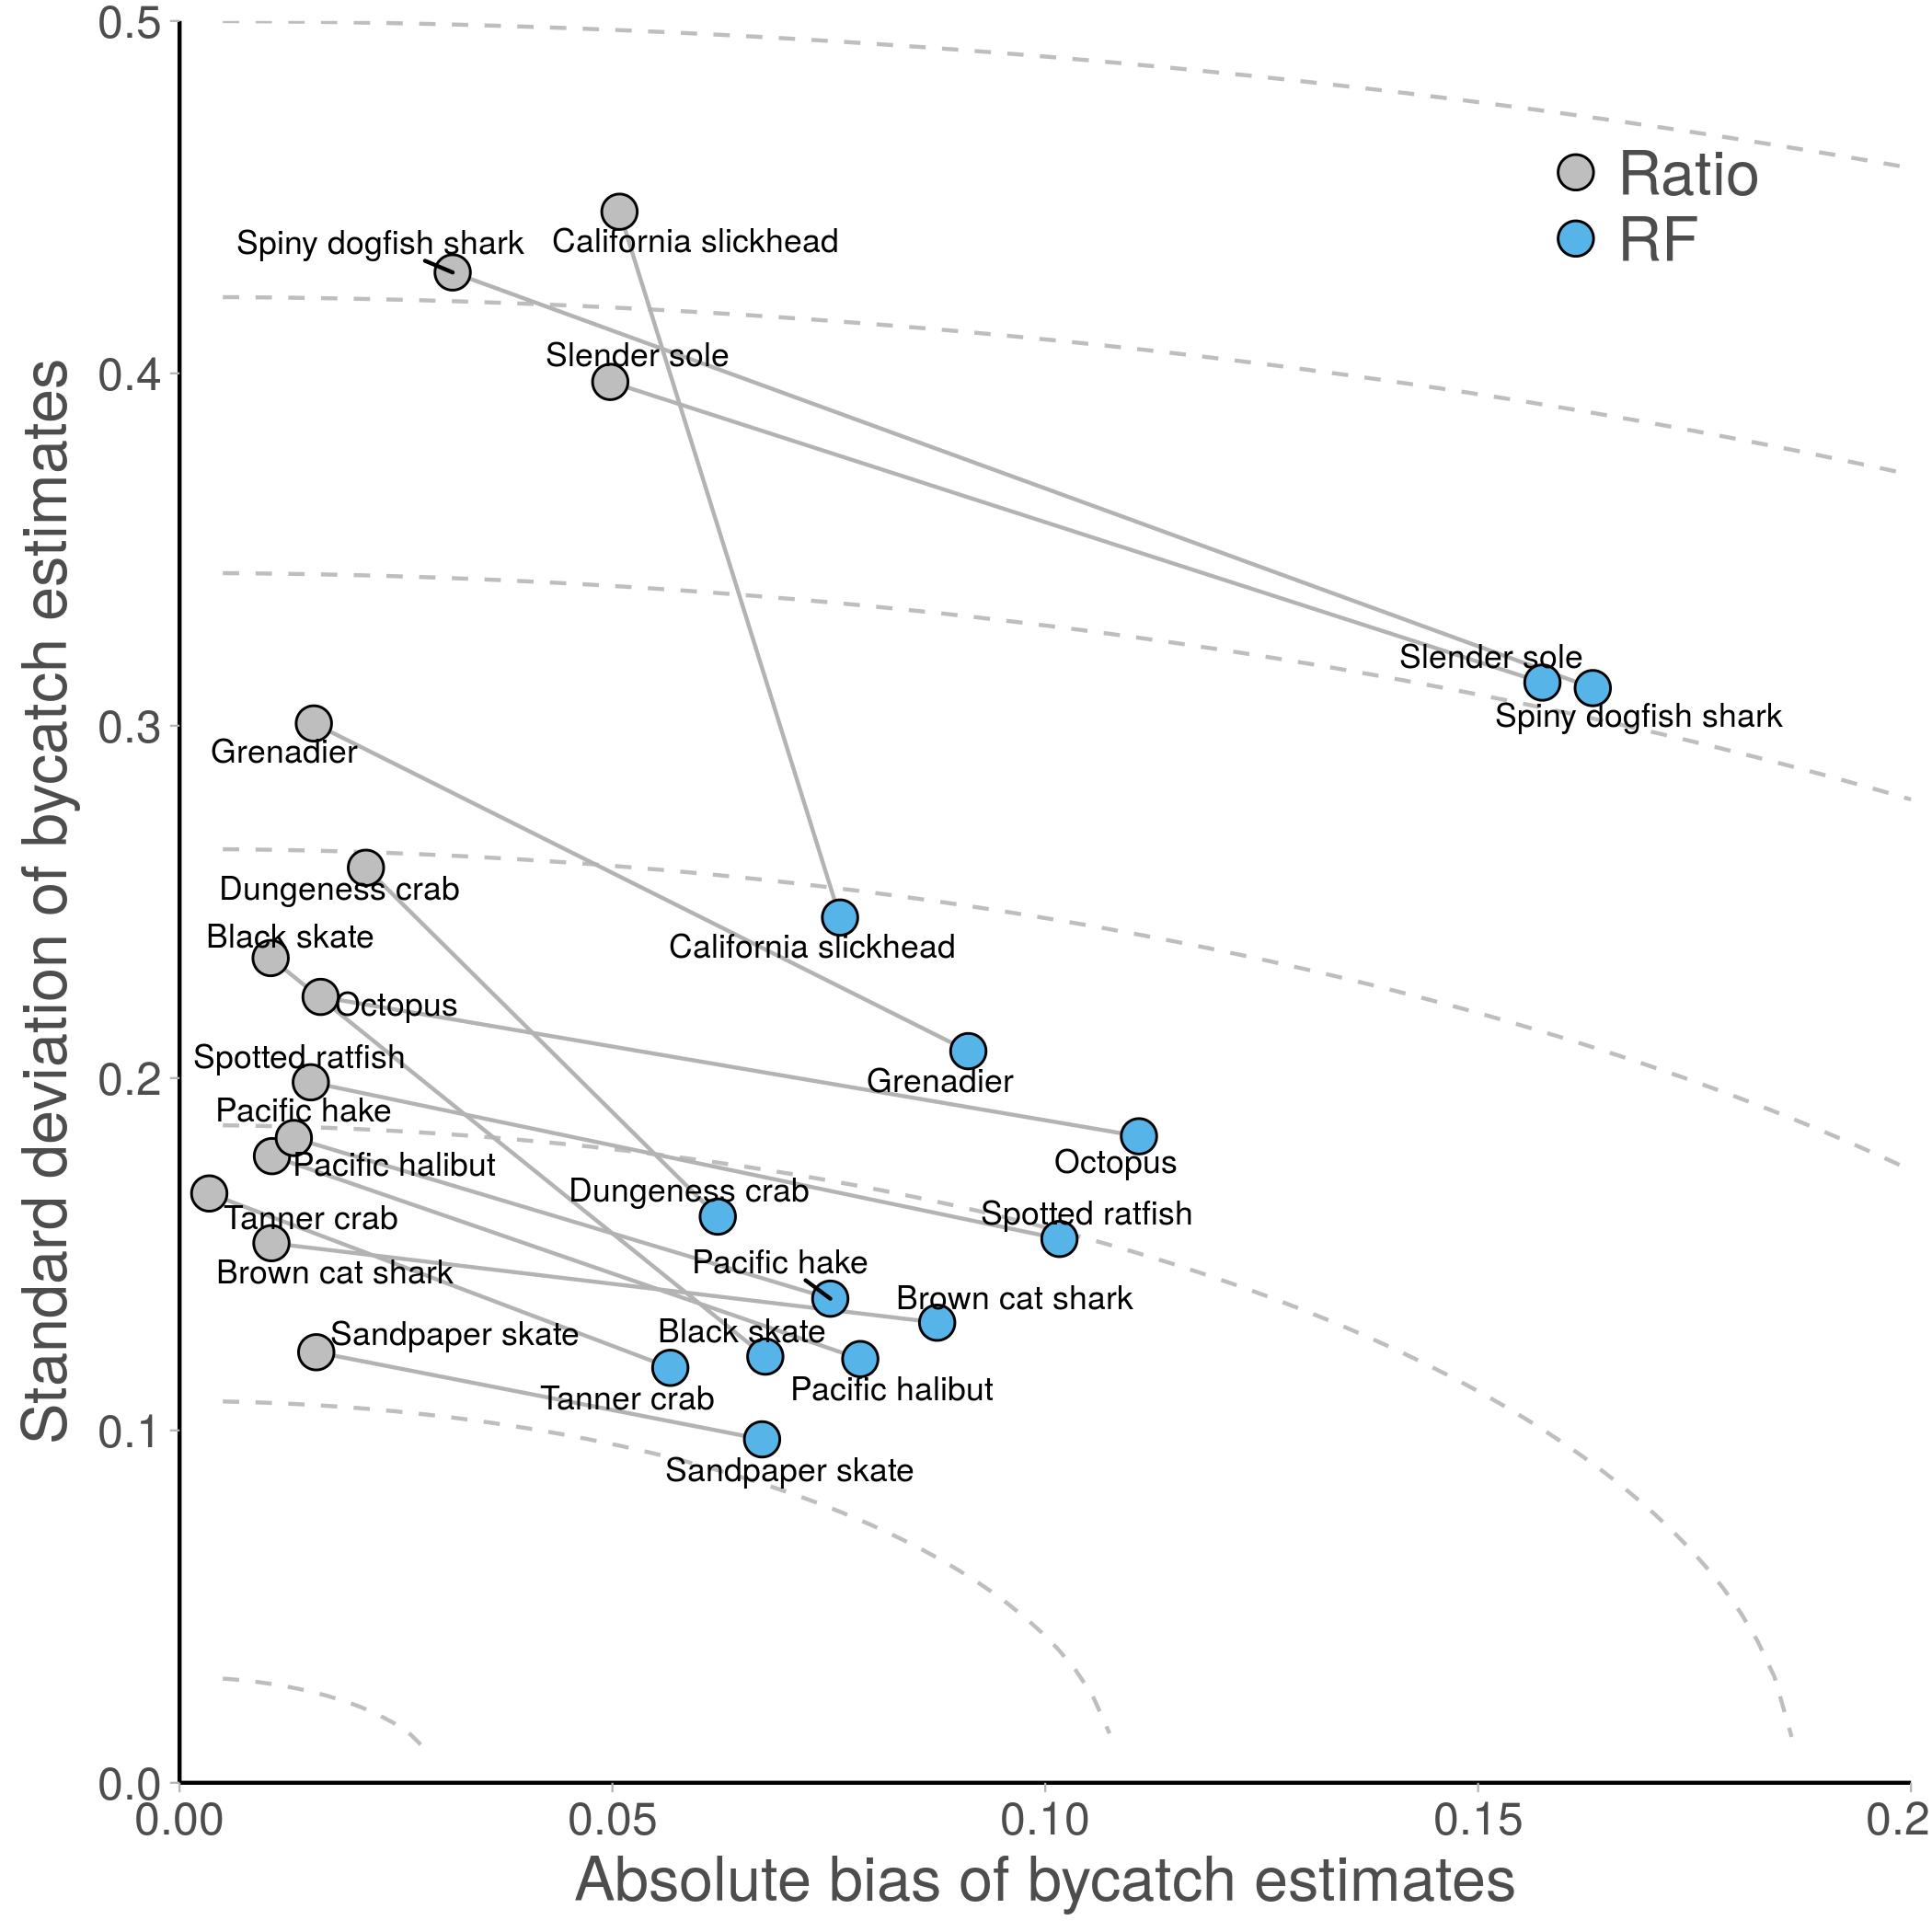
\includegraphics[width=6in]{../figures/supplement/fig7_tradeoffs_v2} 

}

\caption{Bias-variance trade-off between the ratio estimator and RF. RF achieves more accurate predictions (lower RMSE) by allowing some bias but greatly reducing the variance of its estimates. The ratio estimator has very low bias but much higher variance (i.e. it underfits the data and is more sensitive to which hauls are observed). Dashed grey lines indicate iso-RMSE curves. Species with lines that are nearly parallel to the iso-RMSE curves (e.g. Octopus, Brown cat shark) indicate that RF and the ratio estimator perform similarly (same RMSE). Species with lines that cross iso-RMSE curves (e.g. Dungeness crab, California slickhead, Spiny dogfish shark) indicate RF greatly improves on the ratio estimator (lower RMSE). RF has lower RMSE for species with lower bycatch rates (Fig. 11).}\label{fig:variance-bias}
\end{figure}

\pagebreak

\begin{figure}

{\centering 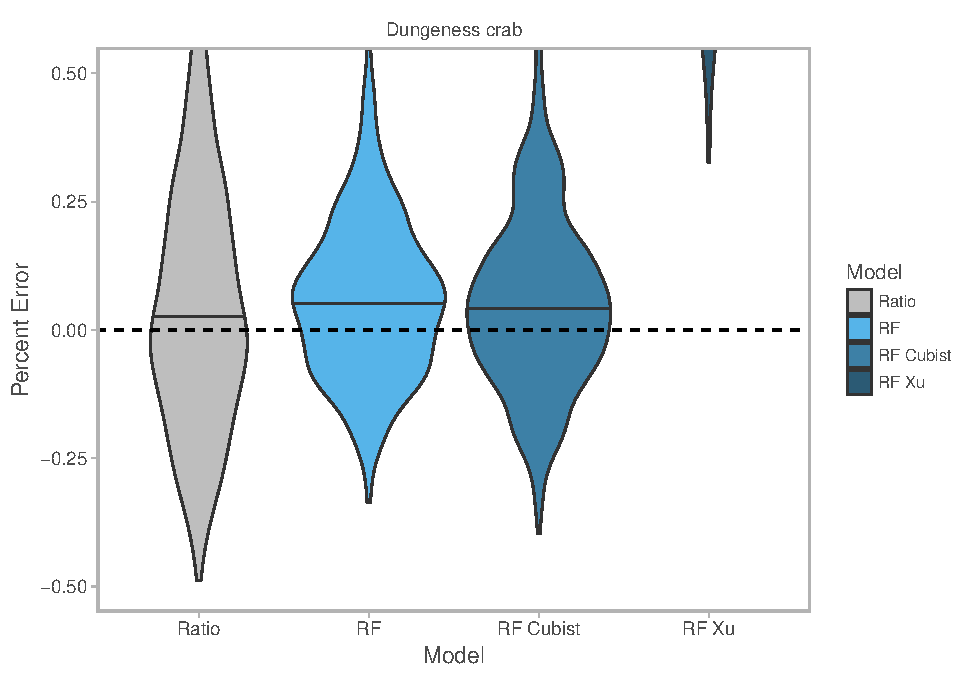
\includegraphics[width=6in]{bycatch_sim_paper_files/figure-latex/rf-cubist-1} 

}

\caption{Performance of RF bias correction methods (percent error, PE, averaged across years 2011-2015). The ratio estimator is unbiased (median PE = 0.002). RF is positively biased (median PE = 0.055) and Cubist is less positively biased (median PE = 0.043). Cubist reduces bias by fitting a linear model in regression tree terminal nodes instead of using the data mean (Quinlan 1992, Quinlan 1993). The second method, Xu (2013), fits a second RF model to the residuals of the original RF, but this method performed poorly (median PE = 1.107, off chart).}\label{fig:rf-cubist}
\end{figure}


\end{document}
